\documentclass[sigconf,anonymous,review,balance=false]{acmart}
\usepackage{popets}
% 추가
\usepackage{cryptocode}
\usepackage{algorithm}
\usepackage{algpseudocode}
\usepackage{amsmath}
\usepackage{enumitem}

\let\Bbbk\relax 
\usepackage{amssymb}

\usepackage{subfig}
\usepackage{amsthm}
\usepackage{booktabs}
\usepackage{multirow}
\usepackage{pgfplots}
\pgfplotsset{compat=1.18}

% Color gradient definitions for multi-spec figures
% Fig 5: Red gradient (Naive) / Blue gradient (Freivalds)
\definecolor{redspec1}{RGB}{240, 140, 140}  % lightest (Tiny)
\definecolor{redspec2}{RGB}{220, 90, 90}    % Mini
\definecolor{redspec3}{RGB}{200, 50, 50}    % Small
\definecolor{redspec4}{RGB}{160, 20, 20}    % Medium
\definecolor{redspec5}{RGB}{110, 0, 0}      % darkest (Base)
\definecolor{bluespec1}{RGB}{120, 170, 240} % lightest (Tiny)
\definecolor{bluespec2}{RGB}{80, 130, 210}  % Mini
\definecolor{bluespec3}{RGB}{50, 100, 190}  % Small
\definecolor{bluespec4}{RGB}{25, 60, 150}   % Medium
\definecolor{bluespec5}{RGB}{0, 25, 100}    % darkest (Base)
% Fig 6: Orange gradient (BERT) / Green gradient (Nystrom)
\definecolor{ornspec1}{RGB}{245, 170, 80}   % lightest (Tiny)
\definecolor{ornspec2}{RGB}{230, 130, 40}   % Mini
\definecolor{ornspec3}{RGB}{200, 100, 10}   % Small
\definecolor{ornspec4}{RGB}{170, 70, 0}     % Medium
\definecolor{ornspec5}{RGB}{120, 45, 0}     % darkest (Base)
\definecolor{grnspec1}{RGB}{100, 190, 120}  % lightest (Tiny)
\definecolor{grnspec2}{RGB}{50, 160, 80}    % Mini
\definecolor{grnspec3}{RGB}{20, 130, 50}    % Small
\definecolor{grnspec4}{RGB}{0, 100, 30}     % Medium
\definecolor{grnspec5}{RGB}{0, 65, 15}      % darkest (Base)

\newcommand{\name}{{\bf zkDietFormer}}
\newcommand{\scheme}{{\bf zkDiet}}
\newcommand{\Q}{{\mathbf{Q}}}
\newcommand{\K}{{\mathbf{K}}}
\newcommand{\V}{{\mathbf{V}}}
\newcommand{\W}{{\mathbf{W}}}
\newcommand{\sfmax}{{\mathrm{softmax}}}
\newcommand{\X}{{\mathbf{X}}}
\newcommand{\Y}{{\mathbf{Y}}}
\newcommand{\Z}{{\mathbf{Z}}}
\newcommand{\F}{{\mathbb{F}}}
\newcommand{\nystrom}{{\text{Nystr\"om }}}
\newcommand{\nystromformer}{{\text{Nystr\"omformer }}}
\newcommand{\rand}{{\mathbf{r}}}

% SNARK
\newcommand{\setup}{{\sf Setup}}
\newcommand{\prove}{{\sf Prove}}
\newcommand{\verify}{{\sf Verify}}
\newcommand{\pk}{{\sf pk}}
\newcommand{\vk}{{\sf vk}}
\newcommand{\ck}{{\sf ck}}
\newcommand{\crs}{{\sf crs}}
\newcommand{\td}{{\sf td}}
\newcommand{\sPi}{{\sf \Pi}}
\newcommand{\bPi}{{\bf \Pi}}
\newcommand{\ins}{{\mathbf{x}}}
\newcommand{\wit}{{\mathbf{w}}}
\newcommand{\comwit}{{\mathbf{u}}}
\newcommand{\uncomwit}{{\mathbf{\omega}}}
\newcommand{\cp}{{\sf cp}}
\newcommand{\cc}{{\sf cc}}


% Commitment
\newcommand{\Com}{{\sf Com}}
\newcommand{\cm}{{\sf cm}}
\newcommand{\commit}{{\sf Commit}}
\newcommand{\kzg}{{\sf KZG}}
\newcommand{\ped}{{\sf Ped}}
\newcommand{\gp}{{\sf gp}}
\newcommand{\comparams}{\textsf{CommitParams}}


% Nystromformer
\newcommand{\selectLandmarks}{{\sf SelectLandmarks}}
\newcommand{\computeMPInverse}{{\sf ComputeMPInverse}}
\newcommand{\NystromAttention}{\textsf{Nystr\"omAttention}}



%common
\newcommand{\R}{{\mathcal{R}}}
\newcommand{\A}{{\mathcal{A}}}
\newcommand{\E}{{\mathcal{E}}}
\newcommand{\sss}[1]{\noindent{\bf #1}.}
\newcommand{\ssi}[1]{\noindent{\it #1}.}
\newcommand{\sample}{{\overset{{\scriptscriptstyle\$}}{\leftarrow}}}

% Security
\newcommand{\negl}{{\sf negl}}

% Copyright
\setcopyright{popets}
\copyrightyear{YYYY}

% Issue info
\acmYear{YYYY}
\acmVolume{YYYY}
\acmNumber{X}
\acmDOI{XXXXXXX.XXXXXXX}
\acmISBN{}
\acmConference{Proceedings on Privacy Enhancing Technologies}
\settopmatter{printacmref=false,printccs=false,printfolios=true}


\begin{document}

%%
%% The "title" command has an optional parameter,
%% allowing the author to define a "short title" to be used in page headers.
\title{\bf \name: Verifiable Transformer Inference with Linear-Cost Attention Proofs via Low-Rank Approximation}

%%%%%%%%%%%%%%%% Authors' Info %%%%%%%%%%%%%%%%%
%%
%% The "author" command and its associated commands are used to define
%% the authors and their affiliations.


%%
%% By default, the full list of authors will be used in the page
%% headers. Often, this list is too long, and will overlap
%% other information printed in the page headers. This command allows
%% the author to define a more concise list
%% of authors' names for this purpose.

\renewcommand{\shortauthors}{Trovato et al.}

%%
%% The abstract is a short summary of the work to be presented in the
%% article.
\begin{abstract}
The widespread deployment of Transformer-based models via Model-as-a-Service platforms raises a fundamental trust problem: users cannot verify that the provider faithfully executed the claimed model on their input. Zero-knowledge SNARKs (zk-SNARKs) can bridge this gap by letting the provider prove correct inference without revealing proprietary model weights, yet existing approaches face an $O(n^2)$ proving-cost bottleneck rooted in the quadratic self-attention mechanism.
        
We propose zkDietFormer, the first zero-knowledge verification framework designed for low-rank self-attention. By instantiating the Nystr\"{o}m approximation inside the proving circuit, we replace the full $n \times n$ attention computation, including the nonlinear cost induced by the row-wise softmax, with three smaller matrix products involving only $m \ll n$ landmark tokens, reducing the dominant cost to $O(n)$. The pseudoinverse factor is supplied as a witness and constrained in-circuit via the Moore--Penrose conditions, avoiding its explicit computation. We further verify large matrix products through Freivalds' single random-vector checks, and employ commit-carrying SNARKs that offload weight commitments outside the circuit while binding every response to a single committed model.
        
Experiments on five BERT-scale configurations (hidden dimensions 128--768, depths 2--12) show that zkDietFormer extends the maximum provable sequence length by up to $4\times$ over standard attention under the same 128\,GB memory budget, with per-layer prove time growing near-linearly in $n$. Under 26-bit fixed-point arithmetic, the quantized model preserves 98.8\% top-1 agreement with its floating-point counterpart.
        
\end{abstract}


%%
%% Keywords. The author(s) should pick words that accurately describe
%% the work being presented. Separate the keywords with commas.
\keywords{Zero-Knowledge Proofs, Verifiable AI, Low-Rank Attention, Transformer, zk-SNARKs}


\maketitle

%-------------------------------------------------------------------------------
\section{Introduction}
%-------------------------------------------------------------------------------
Recent breakthroughs in Transformer-based models have revolutionized artificial intelligence, facilitating the widespread deployment of high-performance Large Language Models (LLMs) via Model-as-a-Service (MaaS) platforms. In this setting, model providers typically large models, while users receive outputs through APIs or remote inference interfaces. However, this architecture inherently obscures the generation process: users cannot independently verify whether the received output truly produced from the specific model architecture and weight parameters intended. Users are therefore forced to rely on trust regarding whether the provider substituted a cheaper model for the same input, post-processed or modified outputs due to internal policies, or unintentionally changed the model during updates or deployment. This problem of model execution integrity is particularly critical in high-stakes domains such as finance, healthcare, and security, and becomes increasingly central as demands for transparency and accountability in inference continue to grow.

One may attempt to address this trust issue by requiring the model provider to disclose model parameters for verification. In practice, however, this is practically infeasible. Model weights are the result of substantial investments in data, compute, and engineering, and are protected as proprietary intellectual property (IP). Consequently, a fundamental dilemma arises: users demand integrity guarantees for the model’s outputs, while providers must preserve the privacy of their model parameters to protect their assets.

Zero-knowledge proofs (ZKPs) provide a principled way to reconcile these conflicting requirements. By leveraging ZKPs, a prover (the model provider) can cryptographically prove that an output $y$ is the result of evaluating the model on the user’s input $x$ with a secret weight $W$, i.e., $f(x, W) = y$, without revealing any information about $W$ itself. This enables verifiable inference while maintaining the confidentiality of model parameters.

However, making ZKP-based verifiable AI practically deployable requires the efficient proving of computationally intensive deep learning operations. In modern Transformer architectures, the primary bottleneck is the self-attention mechanism, the computational core of the model. For an input sequence of length $n$ and hidden dimension $d$, the input $X \in \mathbb{R}^{n \times d}$ is projected into queries, keys, and values $\Q, \K, \V \in \mathbb{R}^{n \times d}$ (for a single attention head). Standard self-attention forms an attention matrix $\Q\K^\top \in \mathbb{R}^{n\times n}$, applies a row-wise softmax over the entire matrix, and then multiplies by $\V$ to obtain the attention output. 

This computation requires $\mathcal{O}(n^2d)$ linear operations for matrix multiplications, as well as an additional $\mathcal{O}(n^2)$ nonlinear cost induced by the softmax. The resulting computational overhead is substantial, posing the single largest obstacle to proving large-scale Transformer models.

The most na\"ive approach to proving self-attention involves arithmetizing the full $\Q\K^\top$ computation into a circuit and enforcing the resulting $\mathcal{O}(n^2 d)$ operations within a SNARK. However, this cost far exceeds practical limits. To mitigate this, many systems have adopted probabilistic verification techniques for large matrix products, such as Freivalds' algorithm~\cite{Freivalds} or Thaler's randomized checks~\cite{Thaler}. These methods verify the $n \times n$ multiplication relation without full recomputation by sampling random vectors, compressing verification to a small number of checks and reducing the cost to $\mathcal{O}(n^2)$. Nevertheless, the complexity remains dominated by the quadratic term, which becomes increasingly prohibitive as models scale. For instance, while BERT~\cite{BERT} uses 512 tokens and GPT-3~\cite{GPT3} uses a 2,048-token context window, frontier models now support contexts in the hundreds of thousands or even millions (e.g., 400K for GPT-5~\cite{GPT5} and 10M for Llama~4 Scout~\cite{llama4}). As $n$ grows, this quadratic verification cost renders proof generation for realistic sequence lengths impractical.

Meanwhile, deep learning literature has repeatedly demonstrated that attention matrices often exhibit an approximate low-rank structure. Concretely, when the number of landmarks $m \ll n$, the attention matrix can be effectively approximated by a rank-$m$ representation, enabling training and inference costs to approach linearity with respect to the sequence length~\cite{Linformer, Nystromformer}. Despite these advances, the field of Verifiable AI has yet to exploit low-rank structures as a primary mechanism for reducing proof generation costs. Consequently, a gap persists: while low-rank approximations improve computational efficiency in practice, the lack of proof systems tailored to these structures keeps proof complexity anchored at $\mathcal{O}(n^2)$. This work aims to bridge this gap. Our central idea is to combine low-rank structures with probabilistic verification to eliminate the quadratic complexity in verifying self-attention matrices.

\subsection{Our Contribution}
In this work, we propose \name, a verification protocol that eliminates the dominant $\mathcal{O}(n^2)$ bottleneck in proving self-attention by combining a low-rank representation of the attention matrix, Freivalds’ randomized checks, and a commit-carrying SNARK. Our main contributions are summarized as follows:
\begin{itemize}
    \item \textbf{The first verification framework tailored to low-rank self-attention.} To the best of our knowledge, we present the first verification framework specifically designed for low-rank self-attention. We instantiate this framework using the \nystrom method, reducing the overall circuit complexity—including both the core matrix operations of self-attention and the nonlinear operations induced by row-wise softmax—to $\mathcal{O}(n)$.
    \item \textbf{Constraint-efficient verification via Freivalds’ checks and CC-SNARKs.} We employ Freivalds’ algorithm to efficiently verify large matrix computations inside the circuit, while leveraging commit-carrying SNARKs to offload computationally expensive operations outside the circuit, significantly reducing the total number of constraints.
    \item \textbf{Practical implementation and evaluation.} We implemented a prototype of the proposed framework and evaluated its performance through benchmarks. The results demonstrate a significant reduction in prover costs for practical sequence lengths, showing that \name is not only theoretically efficient but also practically deployable.
\end{itemize}

In summary, the prover’s constraint cost in \name scales linearly with the input sequence length $n$. Consequently, to the best of our knowledge, this work provides the first verifiable mechanism for low-rank self-attention that enables proof generation with cost linear to the sequence length.



%-------------------------------------------------------------------------------
\section{Related Works}
%-------------------------------------------------------------------------------
% 본 섹션에서는 트랜스포머 모델의 핵심 연산을 간략히 소개하고, 그 중 계산 복잡도의 주요 보틀넥으로 알려진 행렬 곱셈을 효율화시키기 위한 기존 연구들을 살펴본다. 또한 행렬곱 연산에 대하여 zero-knowledge proof를 제공하기 위한 기존 접근법들도 함께 검토한다.
In this section, we provide a brief overview of the core operations of Transformer models and review prior work aimed at improving the efficiency of matrix multiplication, which is widely recognized as a major computational bottleneck. We also examine existing approaches for constructing zero-knowledge proofs for matrix multiplication.

\textbf{Low-Rank Transformer}
% 트랜스포머 모델은 2017년 Google에서 제안된 딥러닝 모델로써, 어텐션 메커니즘을 핵심 구성 요소로 문장 내 단어와 같은 순차적 데이터 간의 관계를 효과적으로 학습한다. 
The Transformer is a deep learning architecture proposed by Google in 2017~\cite{OriginalTransformer}, which leverages the attention mechanism as its core component to effectively model relationships within sequential data, such as words in a sentence. 
% 해당 모델의 핵심 연산은 쿼리(Query), 키(Key), 값(Value)로 구성된 행렬들 간의 행렬 곱셈으로 이루어져 있다. 표준 트랜스포머의 경우, 입력 시퀀스의 길이 n에 따라 이러한 연산은 이차 이상의 계산 복잡도를 가지므로, n이 증가할수록 계산 비용이 급격히 증가한다. 이러한 병목을 완화하기 위해, Child et al은 이미지와 오디오와 같이 주기적인 구조를 가진 데이터에 대해서는 strided attention, 주기적인 구조가 없는 텍스트에 대해서는 fixed attention로 나누어 각각 다른 방식으로 미리 정의된 희소 패턴으로만 토큰을 참고하는 Sparse Transformer를 제안하였다. 특정 텐서플로우 버전에 국한되어있다는 단점이 있었으므로, Longformer는 범용적이고 유지보수가 용이한 각 토큰이 모든 토큰이 아닌 근처 토큰만 참고하는 Sliding Window Attention방식을 제안하였다.  Rae et al은 과거의 은닉 상태를 풀링 함수를 이용해 압축하여 저장하면서, 현재의 세밀한 메모리와 압축된 장기 메모리를 함께 어텐션으로 참조하여 장거리 문맥을 효율적으로 모델링하는 Compressive Transformer를 제안하였다. 그러나 위 방식들은 full attention이 아니어서 장거리 의존성을 정확히 보장하지 못하거나(sparse transformer, Longformer), 속도 향상을 얻는대신 성능이 저하되는(Longformer) 단점을 가진다. 
The core computation of this model consists of matrix multiplications among the query, key, and value matrices. In standard Transformers, these operations incur quadratic computational complexity with respect to the input sequence length n, causing the computational cost to grow rapidly as n increases. To mitigate this bottleneck, Child et al.~\cite{SparseTransformer} proposed the Sparse Transformer, which restricts attention to predefined sparse patterns, using strided attention for data with periodic structures such as images and audio, and fixed attention for text without structure. However, this approach relies on implementations tied to specific TensorFlow versions. To address this limitation, Longformer~\cite{Longformer} introduced sliding-window attention, where each token attends only to nearby tokens, providing a more general and maintainable solution. Rae et al.~\cite{CompressiveTransformer} proposed the Compressive Transformer, which compresses past hidden activations(memories) using pooling operations and jointly attends to both recent memories and compressed long-term memories to efficiently model long-range context. Nevertheless, these approaches do not preserve full attention, leading to limitations such as insufficient modeling of long-range dependencies~\cite{SparseTransformer, Longformer}, or performance degradation in exchange for computational efficiency~\cite{Longformer}.
% 따라서 Linformer는 self-attention으로부터 형성되는 어텐션 행렬이 이론적·경험적으로 저랭크 구조를 가진다는 점을 보이고, 기존의 스케일드 점곱 어텐션에서 키와 값 행렬을 선형 투영을 통해 저차원 공간으로 사상함으로써 어텐션 연산을 저랭크로 근사하였다. 이를 통해 시퀀스 길이 n에 대해 self-attention의 시간 및 공간 복잡도를 선형으로 감소시켰다.
Accordingly, Linformer~\cite{Linformer} shows that the attention matrix induced by self-attention exhibits a low-rank structure both theoretically and empirically, and approximates scaled dot-product attention by projecting the key and value matrices into a lower-dimensional space via linear projections. As a result, the time and space complexity of self-attention are reduced to linear in the sequence length n.
% 그러나 Linformer가 미래 토큰을 가려야 하는 인과적(Causal) 모델링이 어렵고, 실제 어텐션과의 오차가 크다는 단점이 있어, Performer는 별도의 투영 행렬이나 저차원(low-rank) 가정에 의존하지 않고, 무작위 가우시안 투영 함수 기반의 커널화 기법인 FAVOR+를 통해 소프트맥스 연산을 수학적으로 분해함으로써 정규 어텐션과 근사한 효과를 내는 선형 복잡도의 어텐션을 제안하였다.
However, Linformer has limitations in causal modeling, where future tokens must be masked, and can incur large mean squared errors compared to exact attention. To overcome these issues, Performer~\cite{Performer} introduces a linear-complexity attention mechanism that avoids explicit projection matrices and low-rank assumptions, and instead approximates full softmax attention via FAVOR+, which is based on positive orthogonal random features for softmax kernel estimation.
% Nystromformer는 일부 핵심 토큰(Landmarks)의 조합으로 전체 어텐션 맵을 재구성하는 Nyström 저차원 근사 기법을 도입하여, 기존 Performer 등의 선형 어텐션 모델보다 높은 정확도를 달성하면서도 시퀀스 길이에 비례하는 선형 복잡도를 유지하였다.
Nyströmformer~\cite{Nystromformer} introduces a Nyström low-rank approximation that reconstructs the full attention map using a subset of landmark tokens, achieving higher accuracy than Performer while maintaining linear complexity with respect to the sequence length.

\textbf{zk-SNARKs for Matrix Multiplication}
% 물론 환원 가능하더라도 합성곱 연산은 행렬곱과 다르기 때문에 행렬곱 위주로 작성
% 행렬 곱셈의 무결성을 영지식 증명을 통해 검증하려는 연구는 지속적으로 이루어져 왔다. 합성곱 연산은 구조화된 행렬 곱셈으로 환원될 수 있으므로, 영지식 증명을 이용한 행렬 곱셈 무결성 검증은 AI 모델 실행의 정확성과 무결성을 증명하기 위한 핵심 기술로 꾸준히 연구되어 왔다.
There has been ongoing research on verifying the integrity of matrix multiplication using zero-knowledge proofs. Since convolution operations can be reduced to structured matrix multiplication, such verification techniques have been extensively studied as a core technique for proving the correctness and integrity of AI model execution.

% Justin Thaler는 행렬 곱셈 검증을 위해 Sumcheck 프로토콜에 reuse-of-work 기법을 적용함으로써, n \times n 행렬 곱에서 증명자의 계산 오버헤드를 기존의 O(n^3)에서 O(n^2)로 줄였다. zkCNN은 Fully connected layer의 행렬 곱 연산을 검증하기 위해 이러한 최적화된 합계 체크 기법을 활용하였다.
Thaler et al.~\cite{Thaler} introduced the reuse-of-work technique into the Sumcheck protocol for matrix multiplication verification, reducing the prover’s computational overhead from $O(n^3)$ to $O(n^2)$ for $n \times n$ matrices. zkCNN~\cite{zkCNN} adopts this optimized Sumcheck protocol to efficiently verify matrix multiplication in fully connected layers.
% pvCNN~\cite{pvCNN}은 필터와 입력을 사각 행렬로 바꾸어, 수많은 곱셈 게이트가 필요한 컨볼루션(합성곱) 연산을 단 하나의 행렬곱 연산으로 표현한 뒤, vCNN~\cite{vCNN}이 QAP에 다항식을 적용한 QPP(Quadratic Polynomial Programs) 방식에서 영감을 얻어, 이를 확장한 QMP(Quadratic Matrix Program)를 통해 단 하나의 곱셈 게이트만으로 계산하였다.
pvCNN~\cite{pvCNN} transforms convolution operations, which inherently require a large number of multiplication gates, into a single matrix multiplication by reshaping the filters and inputs into rectangular matrices. Inspired by the QPP (Quadratic Polynomial Programs) approach of vCNN~\cite{vCNN}, which applies polynomial representations within the QAP framework, pvCNN further extends this idea by introducing the QMP (Quadratic Matrix Program). As a result, the convolution can be expressed and verified using only a single multiplication gate.
% zkML~\cite{zkML}은 convolutions, batched matrix multiplication와 같은 linear layer에서 처리하는 행렬곱 연산에 대하여 프리발드 알고리즘~\cite{Freivalds}을 적용하여 O(n^2)의 복잡도로 검증하였다.
zkML~\cite{zkML} applies Freivalds’ algorithm~\cite{Freivalds} to verify matrix multiplication operations in linear layers, such as convolutions and batched matrix multiplications, achieving verification complexity of $O(n^2)$.
% zkLLM~\cite{}은 트랜스포머 모델에서 발생하는 행렬 곱 연산을 증명하기 위해, SafetyNets ~\cite{}에서 행렬 곱 검증을 목적으로 설계된 dedicated sumcheck 프로토콜을 활용하였다. 이로 인해 증명자 계산 시간은 두 입력 행렬의 크기에 비례하는 O(mn + np)의 계산 복잡도를 가진다.
% zkLLM~\cite{zkLLM} leverages the dedicated sumcheck protocol proposed in SafetyNets~\cite{SafetyNets} to verify matrix multiplication operations arising in Transformer models. As a result, the prover’s computational complexity scales linearly with the sizes of the input matrices, achieving a complexity of $O(mn+np)$.
zkLLM~\cite{zkLLM} employs specialized sumcheck protocols for tensor operations, achieving prover complexity linear in the total tensor size $O(D)$, together with tlookup and zkAttn for non-arithmetic operations such as softmax. This line of work builds on the interactive-proof approach to neural network verification introduced by SafetyNets~\cite{SafetyNets}, which applies GKR-based protocols to matrix multiplication in arithmetic-circuit-representable networks. 
% zkMatrix~\cite{zkMatrix}은 행렬 곱셈을 네 개의 내적 관계(inner-product relations)로 환원하고 Bulletproofs 기반의 검증 가속화 기법을 적용함으로써, n \times n 커밋 행렬 곱셈에 대해 증명자 시간O(n^2) 검증자 시간 O(log⁡n)을 제공하였다.
% zkMatrix~\cite{zkMatrix} reduces matrix multiplication to four inner-product relations and applies Bulletproofs-based verification acceleration techniques, thereby achieving a prover time of $O(n^2)$ and a verifier time of $O(\log n)$ for $n \times n$ committed matrix multiplication.
zkMatrix~\cite{zkMatrix} applies Bulletproofs-based acceleration to committed matrix multiplication, achieving $O(n^2)$ prover time with $O(\log n)$ verifier time and transcript size for $n \times n$ matrices, and reducing the marginal cost of each additional multiplication to $O(n)$ group operations under batching.

% 그러나 이러한 방식들은 여전히 행렬 차원(또는 시퀀스 길이)에 대해 O(n^2)의 증명자 계산 복잡도를 요구하거나~\cite{Thaler, zkCNN, vCNN, zkML, zkMatrix}, 이론적으로 선형 시간 복잡도를 달성하더라도 행렬을 구성하는 다른 차원 m 자체가 매우 크다는 한계를 지닌다~\cite{zkLLM}. 또한 SoftMax와 같은 비선형 함수를 ZKP 회로 내에서 직접 처리할 수 없어 근사 기법에 의존해야 하며, 이로 인해 정확도 손실이 발생하고 ZKP에 특화된 새로운 모델 구조를 설계해야 한다는 제약이 존재한다~\cite{zkVC}.

However, these approaches still require a prover computation complexity of $O(n^2)$ with respect to the matrix dimension (or sequence length)~\cite{Thaler, zkCNN, vCNN, zkML, zkMatrix}, or, even when achieving linear-time complexity in theory, suffer from the limitation that the other matrix dimension m remains prohibitively large in practice~\cite{zkLLM}. Moreover, nonlinear functions such as softmax cannot be directly handled within ZKP circuits and thus must be approximated, which leads to accuracy degradation and necessitates the design of model architectures specifically tailored for zero-knowledge proof systems~\cite{zkVC}.

%-------------------------------------------------------------------------------
\section{Preliminaries}
\label{sec:preliminaries}
%-------------------------------------------------------------------------------

\sss{Notation}
We denote the sequence length by $n$, the hidden dimension by $d$, and the per-head query/key and value dimensions by $d_k$ and $d_v$, respectively. The number of attention heads is $h$, the number of Transformer layers is $L$, and the number of landmarks is $m$, giving a segment length $\ell = n/m$. The circuit precision parameter $k_{\text{bits}}$ controls the bit-width of quantized fixed-point arithmetic. %(unrelated to the landmark count $m$). %Matrices in the plaintext model are over the real field $\mathbb{R}$; after quantization for the ZK circuit, they are over the finite field $\mathbb{F}$.

% 트랜스포머 모델은 각 단어 간 상호작용을 차원이 d_k인 query와 key, 그리고 차원이 d_v인 value로 표현한다. 각 쿼리는 문장 내의 다른 토큰들에 대응하는 키와의 유사도를 계산하고, 현재 토큰이 어떤 정보에 더 집중해야 하는지를 결정한다. 이후 이러한 유사도를 기반으로 값의 가중합을 계산함으로써 문맥 정보를 통합한다.
% 어텐션 함수는 하나의 쿼리와 키–값 쌍들의 집합을 입력으로 받아 출력 벡터를 생성하는 함수로 정의되며, 이때 쿼리, 키, 값, 그리고 출력은 모두 벡터 공간 상에 존재한다. 실제 구현에서는 여러 개의 쿼리를 동시에 처리하기 위해 이를 행렬 형태로 묶어 Q, K, V로 표현하여 한 번에 계산한다.
% 구체적으로, 어텐션 가중치는 쿼리와 키의 내적을 $1/\sqrt{d_k}$ 로 스케일링한 후 소프트맥스 함수를 적용하여 계산되며, 최종 출력은 해당 가중치에 따른 값 벡터들의 가중합으로 산출된다.
\subsection{Scaled Dot-Product Attention}
The model represents interactions between tokens using queries and keys of dimension $d_k$, and values of dimension $d_v$. For each token, its associated query computes its similarity scores with the keys of all other tokens in the sequence, thereby determining which parts of the input the model should attend to more strongly. The contextual information is then aggregated by computing a weighted sum of the corresponding value vectors based on these similarities.

The attention mechanism is defined as a function that takes a single query together with a set of key–value pairs and produces an output vector, where the query, keys, values, and outputs all lie in vector spaces. In practice, multiple queries are processed simultaneously by stacking them into matrices $\Q$, $\K$, and $\V$. These matrices are obtained by projecting the input matrix $\X \in \mathbb{R}^{n \times d}$ using learnable parameter matrices $\W^Q \in \mathbb{R}^{d \times d_k}$, $\W^K \in \mathbb{R}^{d \times d_k}$, and $\W^V \in \mathbb{R}^{d \times d_v}$, yielding $\Q = \X \W^Q \in \mathbb{R}^{n \times d_k}$, $\K = \X \W^K \in \mathbb{R}^{n \times d_k}$, and $\V = \X \W^V \in \mathbb{R}^{n \times d_v}$. Concretely, the attention weights are obtained by scaling the dot product between queries and keys by $1/\sqrt{d_k}$, followed by the application of the softmax function. The final output is computed as the weighted sum of the value vectors using these attention weights.

The output matrix is computed as follows:
\[
    \text{Attention} (\Q, \K, \V ) = \sfmax\left(\frac{\Q\K^\top}{\sqrt{d_k}}\right)\V
\]


\subsection{Multihead Attention}
% 멀티헤드 어텐션은 단일 어텐션 함수에서 d_model-차원의 키,값, 쿼리를 사용하는 대신, 쿼리, 키, 값을 각각 h회에 걸쳐 서로 다른 학습된 선형 변환을 통해 차원 d_k, d_k, d_v로 linear projection한 뒤, 각 헤드에서 병렬적으로 어텐션을 수행한다. 구체적으로, 각 헤드 i에 대해 다음과 같이 정의된다:
% \text{head}_i = \attn (\Q W_i^{Q},\K W_i^{K}, \V W_i^{V}),
% 여기서 W_i^{Q} \in \mathbb{R}^{d_{\text{model}}\times d_k}, W_i^{K} \in \mathbb{R}^{d_{\text{model}}\times d_k}, W_i^{V} \in \mathbb{R}^{d_{\text{model}}\times d_v}는 학습 가능한 투영 행렬이다.

% 각 헤드의 출력은 연결(concatenate)된 후 다시 원래 차원으로 선형 변환된다:
% MultiHead(Q,K,V)=Concat(head1,...,headh)WO
% 여기서 W^{O} \in \mathbb{R}^{h d_v \times d_{\text{model}}}이다.
% 이와 같은 구조는 각 헤드가 서로 다른 표현 패턴과 의미적 하위공간에 집중하도록 하며, 동시에 이 정보를 통합할 수 있게 한다. 또한 각 헤드에서 차원을 d_{\text{model}}/h 수준으로 축소함으로써, 전체 계산 비용은 단일 헤드 어텐션과 유사한 수준으로 유지된다.
Multi-head attention replaces a single attention function over $d$-dimensional queries, keys, and values with $h$ parallel attention heads. The queries, keys, and values are first linearly projected $h$ times into lower-dimensional subspaces of sizes $d_k$ and $d_v$, respectively. For each head $i$,
\[
    \text{head}_i = \text{Attention} (\Q_i, \K_i, \V_i)
\]
where $\Q_i = \X \mathbf{W}_i^{Q}$, $\K_i = \X \mathbf{W}_i^{K}$, $\V_i = \X \mathbf{W}_i^{V}$, with learnable projection matrices $\mathbf{W}_i^{Q} \in \mathbb{R}^{d\times d_k}, \mathbf{W}_i^{K} \in \mathbb{R}^{d\times d_k}$, and $\mathbf{W}_i^{V} \in \mathbb{R}^{d\times d_v}$.
The resulting head outputs are concatenated and linearly transformed to form the final representation:
\[
\text{MultiHead}(\Q,\K,\V)=\text{Concat} (\text{head}_1,\dots,\text{head}_h) \mathbf{W}^{O}
\]
with $\mathbf{W}^{O} \in \mathbb{R}^{h d_v \times d}$.
In the standard setting, $d_k = d_v = d/h$, so that the total cost across heads matches that of single-head attention over $d$ dimensions. This design enables the model to attend to diverse representation subspaces while maintaining computational cost comparable to single-head attention. For clarity, we describe the protocol for a single attention head with $d_k = d_v = d$; the extension to $h$ heads follows by applying the same construction per head.

\subsection{Nystrom-Based Linear Attention}\label{subsec:nystrom-linear}
% 나이스트롬 트랜스포머는 행렬 근사(matrix approximation)에서 널리 쓰이는 나이스트롬 method~\cite{}를 적용하여, 기존 트랜스포머의 계산 복잡도를 O(n^2)에서 O(n)으로 줄인다. 나이스트롬 방식의 핵심은 행렬 전체를  직접 계산하는 대신, 일부 열과 행만을 사용하여 전체 행렬을 근사적으로 재구성하는 것이다.
%아래 식의 좌측과 같이 소프트맥스 행렬 S를 블록 행렬로 표현할 때, 나이스트롬 방식은 우측과 같이 계산 비용이 큰 $C_S \in R^{(n−m)×(n−m)}$를 $A_S \in R^{m \times m}, B_S \in R^{m×(n−m)}, F_S \in R^{(n−m)×m}로 근사하여 표현한다.
% 식써주고
% 여기서 $A_S^+$는 Moore-Penrose 유사역행렬이다.
% 하지만 이 방식을 셀프 어텐션에 직접 적용할 경우, Softmax의 행별 정규화 특성 상 분모를 계산하기 위해 여전히 $n \times n$ 크기의 행렬 전체에 접근해야 하는 문제가 발생한다. 이를 해결하기 위해 Nyströmformer는 Softmax를 적용하기 전에  전체 시퀀스를 $m$개의 구간으로 나누고, 각 구간의 평균값을 취해 Query와 Key에서 각각 $m$개의 랜드마크($\tilde{Q}, \tilde{K}$)를 생성 한 뒤, 이를 바탕으로 세개의 저차원 행렬을 구성한다. 
% 이러한 행렬을 이용하여 Nystromformer는 선형 복잡도를 가지는 다음의 최종 근사식을 얻는다.
% 식 써주고 
% 식 중앙의 유사역행렬 A^+_S을 계산하는 일반적인 방식(예:SVD)은 GPU 연산 효율이 낮아 실제 구현에 병목이 된다. 따라서 Nyströmformer는 단순 행렬 곱셈을 반복하여 유사역행렬을 빠르게 근사하는 알고리즘을 도입하였으며, 여기서 도출된 $Z^*$를 최종 식에 대입하여 연산 속도를 극대화하였다.
Nyströmformer applies the Nyström method~\cite{Nystromformer}—a technique widely used in matrix approximation—to reduce the computational complexity of the standard Transformer from $O(n^2)$ to $O(n)$. The key idea of the Nyström method is to reconstruct the full matrix approximately by using only a subset of its rows and columns, instead of computing the entire matrix explicitly.

When the softmax matrix $S$ is expressed as a block matrix as shown below, 
\[
    S = \sfmax(\frac{\Q\K^\top}{\sqrt{d_k}}) = \begin{bmatrix} A_S\ B_S \\ F_S\ C_S \end{bmatrix}
\]
the Nystrom method approximates the expensive block $C_S \in \mathbb{R}^{(n-m)\times (n-m)}$ by using the smaller blocks $A_S \in \mathbb{R}^{m \times m}, B_S \in \mathbb{R}^{m \times (n-m)}, F_S \in \mathbb{R}^{(n-m)\times m}$ as illustrated below:
\[
    \hat S = \begin{bmatrix}
            A_S & B_S \\
            F_S & F_S A_S^{+} B_S
            \end{bmatrix} =
            \begin{bmatrix}
            A_S \\
            F_S
            \end{bmatrix}
            A_S^{+}
            \begin{bmatrix}
            A_S & B_S
            \end{bmatrix}
\]
Here, $A_S^+$ denotes the Moore-Penrose pseudoinverse of $A_S$.

However, when this approach is applied directly to self-attention, the row-wise normalization property of the softmax function still requires accessing all entries of the $n \times n$ matrix in order to compute the denominators. To address this issue, Nyströmformer partitions the entire sequence into $m$ segments of length $\ell = n/m$ before applying softmax, and computes the mean within each segment to obtain $m$ landmark points for the queries and keys, respectively. These landmarks yield $\widetilde{\Q}, \widetilde{\K} \in \mathbb{R}^{m \times d}$, from which three low-rank factors $\Q\widetilde{\K}^\top \in \mathbb{R}^{n \times m}$, $\widetilde{\Q}\widetilde{\K}^\top \in \mathbb{R}^{m \times m}$, and $\widetilde{\Q}\K^\top \in \mathbb{R}^{m \times n}$ are formed. The resulting factors play the same structural role as $\begin{pmatrix} A_S \\ F_S \end{pmatrix}$, $A_S^{+}$, and $\begin{pmatrix} A_S & B_S \end{pmatrix}$ in the block decomposition above, but are computed from landmarks rather than extracted from~$S$.
Using these matrices, Nyströmformer derives a final approximation that achieves linear computational complexity:

\begin{align*}
\hat S V &=
\sfmax\!\left(\frac{\Q\widetilde{\K}^{\top}}{\sqrt{d_k}}\right)
\,
\sfmax\!\left(\frac{\widetilde{\Q}\widetilde{\K}^{\top}}{\sqrt{d_k}}\right)^{+}
\,
\sfmax\!\left(\frac{\widetilde{\Q}\K^{\top}}{\sqrt{d_k}}\right)V
\end{align*}

The exact computation of the pseudoinverse $A_S^{+}$ (e.g., via SVD) is computationally expensive and poorly suited for GPU execution, becoming a practical bottleneck in implementation. To mitigate this issue, Nyströmformer introduces an iterative algorithm that approximates the pseudoinverse using repeated matrix multiplications. The resulting approximation $Z^*$ is then substituted into the final formulation, significantly improving computational efficiency.

\begin{align*}
\hat S V &= \sfmax\!\left(\frac{\Q\widetilde{\K}^{\top}}{\sqrt{d_k}}\right)\, Z^* \,
\sfmax\!\left(\frac{\widetilde{\Q}\K^{\top}}{\sqrt{d_k}}\right)V
\end{align*}

\subsection{zk-SNARKs}
A \textit{zero-knowledge succinct non-interactive argument of knowledge}(zk-SNARKs) for an NP relation $\R$ consists of three PPT algorithms $\Pi$ = $(\setup, \prove, \verify)$:
\begin{itemize}
    \item $(\pk, \vk) \gets \Pi.\setup(1^\lambda, \R)$: On input the security parameter $\lambda$ and a relation $\R$, the setup algorithm outputs a proving key $\pk$ and a verification key $\vk$.
    \item $\pi \gets \Pi.\prove(\pk, \ins; \wit)$: On input the proving key $\pk$, a statement $\ins$, and a witness $\wit$ such that $(\ins, \wit) \in \R$, the prover outputs a proof $\pi$.
    \item $0/1 \gets \Pi.\verify(\vk, \ins, \pi)$: On input the verification key $\vk$, a statement $\ins$, and a proof $\pi$, the verifier outputs 0(reject) or 1(accept)
\end{itemize}
A zk-SNARK system $\Pi$ satisfies the following properties:

\ssi{Completeness} For every true statement for the relation $\R$, an honest prover holding a valid witness always convinces the verifier, i.e., $\forall(\ins, \wit) \in \R$:
    \begin{equation*}
        \Pr\left[
        \begin{matrix}
            \begin{gathered}
                (\pk, \vk) \gets \Pi.\setup(1^\lambda, \R) \\
                \pi \gets \Pi.\prove(\pk, \ins; \wit)
            \end{gathered} 
            : & 
            \begin{gathered}
                \Pi.\verify(\vk, \ins, \pi) =1
            \end{gathered}
        \end{matrix}
        \right] = 1
    \end{equation*}

\ssi{Knowledge Soundness} Knowledge soundness requires that any prover producing a proof $\pi$ that makes the verifier accept must possess a corresponding witness, and that a knowledge extractor $\mathcal{E}$ can efficiently extract such a witness from $\pi$. Formally, for any PPT adversary $\mathcal{A}$, the following is \textit{negligible}.
\begin{equation*}
\Pr\left[
\begin{aligned}
     \quad & (\pk, \vk) \gets \Pi.\setup(\R) & & \Pi.\verify(\vk, \ins^*, \pi^*) = 1\\
     &  (\ins^*, \pi^*) \gets \A(\pk, \vk) &:\quad & \wedge \\
     & \wit \gets \E_\A(trans_\A) & & (\ins^*; \wit) \notin \R \quad \quad
\end{aligned}
\right]
\end{equation*}

\ssi{Zero-Knowledge}
There exists a PPT simulator $\mathcal{S} = (\mathcal{S}_1, \mathcal{S}_2)$ such that $\mathcal{S}_1$ outputs simulated setup parameters $(\pk, \vk)$ together with a trapdoor $td$. On input $(\pk, \vk, td), \mathcal{S}_2$ outputs a simulated proof $\pi$. Moreover, for all PPT adversaries $\mathcal{A} = (\A_1, \A_2)$, we have that
\begin{align*}
    &\left|
    \Pr\!\left[
      \A_2(\vk, \ins, \pi) = 1 :
      \begin{array}{l}
        (\pk,\vk)\leftarrow \Pi.\setup(1^\lambda, \R) \\
        (\ins, \wit) \gets \A_1(1^\lambda, \pk, \vk) \\
        \pi\leftarrow \Pi.\prove(\pk, \ins; \wit)
      \end{array}
    \right]
    \right. \nonumber\\
    &\left.
    -
    \Pr\!\left[
      \A_2(\vk, \ins, \pi) = 1 :
      \begin{array}{l}
        (\pk,\vk,td)\leftarrow \mathcal{S}_1(1^\lambda, \R) \\
        (\ins, \wit) \gets \A_1(1^\lambda, \pk, \vk) \\
        \pi\leftarrow \mathcal{S}_2(\pk, \ins, td)
      \end{array}
    \right]
    \right|
    \le \negl(\lambda).
\end{align*}

\ssi{Succinctness} For any statement $\ins$ and witness $\wit$, the size of proof $\pi$ satisfies $|\pi| = poly(\lambda)\cdot polylog(|\ins| + |\wit|)$ \\


\sss{Commit-and-Prove SNARKs (CP-SNARKs)}
A \textit{Commit-and-Prove SNARKs} (CP-SNARKs)~\cite{Legosnark, Lunar} allow a prover to prove statements about values hidden in a commitment. Let $\Com$ be a commitment scheme. Given a commitment $\cm$ to $\comwit$, a CP-SNARK proves knowledge of a witness $\wit$ consistent with $\cm$ and satisfying a relation $\R$. Formally, for $\R(\ins;\wit)$, we write $\wit := (\uncomwit, \comwit, o)$, where $\comwit$ is committed, $\uncomwit$ is uncommitted, and $o$ is the opening randomness, such that $\cm=\Com(\comwit; o)$ and $\R(\ins; \wit)=1$. A CP-SNARK is a tuple of algorithms $\Pi_{\cp}=(\setup,\prove,\verify)$.
\begin{itemize}
    \item $(\pk, \vk) \gets \Pi_\cp.\setup(1^\lambda, \R, \ck)$: Same as $\Pi.\setup$, but additionally takes the commitment key $\ck$ as input.
    \item $\pi_{\cp} \gets \Pi_\cp.\prove(\pk, \ins; \wit)$:
    Equal to $\Pi.\prove(\pk, \{\ins,\cm\};\{\comwit,o\}, \uncomwit)$.
    It is based on $\Pi.\prove$, but additionally takes the commitment $\cm$ as input, and the witness includes the committed value $\comwit$ and its opening $o$, together with the uncommitted part $\uncomwit$.
    \item $0/1 \gets \Pi_\cp.\verify(\vk, \ins, \cm, \pi_\cp)$ Same as $\Pi.\verify$, except that it additionally takes $\cm$ as input.
\end{itemize}

\sss{Commit-Carrying SNARKs (CC-SNARKs)}
A \textit{Commit-Carrying SNARKs} (CC-SNARKs)~\cite{Legosnark, Vectis} extend the commit-and-prove approach by generating the witness commitment during proving. This helps scale to large circuits by moving expensive computations (e.g., group exponentiation) outside the circuit: the prover commits using a circuit-dependent key $\ck$, and the resulting commitment $\cm$ is carried into the verification equation. A cc-SNARK consists of three PPT algorithms $\Pi_{\cc}=(\setup,\prove,\verify)$.

\begin{itemize}
    \item $(\ck, \pk, \vk) \gets \Pi_\cc.\setup(1^\lambda, \R)$: Similar to $\Pi_\cp.\setup$, but additionally outputs the circuit-dependent commitment key $\ck$ together with $(\pk,\vk)$.
    \item $(\pi_\cc, \tilde{\cm}) \gets \Pi_\cc.\prove(\pk, \ins; \wit, \tilde{o})$: The witness is partitioned as $\wit := (\comwit,\uncomwit)$ into a committed part and an uncommitted part.
    The prover outputs a proof $\pi_\cc$ together with a proof-dependent commitment $\tilde{\cm} =\Com.\commit(\ck, \comwit; \tilde{o})$.
    \item $0/1 \gets \Pi_\cc.\verify(\vk, \ins, \tilde{\cm}, \pi_\cc)$: On input the verification key $\vk$, a statement $\ins$, a proof-dependent commitment $\tilde{\cm}$, and a proof $\pi_\cc$, the verifier outputs 0(reject) or 1(accept)
\end{itemize}


\subsection{Freivalds’ Algorithm}
Freivalds' algorithm~\cite{Freivalds, Korec} is a simple yet powerful randomized method for verifying a matrix product without recomputing it.
Let \(\X,\Y,\Z\in \mathbb{F}^{n\times n}\) and consider the claim \(\X \cdot \Y=\Z\).
Instead of computing \(\X\Y\) in \(\mathcal{O}(n^3)\) time, Freivalds samples a uniformly random vector \(\mathbf{r}\sample \mathbb{F}^n\) and checks
\[
\X(\Y\mathbf{r}) \stackrel{?}{=} \Z\mathbf{r}.
\]
This verification runs in \(\mathcal{O}(n^2)\) field operations. This algorithm has soundness error: if \(\X\Y=\Z\), it always accepts.
Otherwise, when \(\X\Y\neq \Z\), the check passes with probability at most \(1/|\mathbb{F}|\), i.e.,
\[
\Pr\!\big[\,\X(\Y\mathbf{r}) = \Z\mathbf{r}\ \big|\ \X\Y\neq \Z\,\big] \le \frac{1}{|\mathbb{F}|}.
\]
The same principle extends to rectangular matrices and to the transposed (left-multiplied) variant $\mathbf{r}^{\top}\!\X\Y \stackrel{?}{=} \mathbf{r}^{\top}\!\Z$, which we use in Section~\ref{sec:protocol} to verify products of varying dimensions.

%-------------------------------------------------------------------------------
\section{Technical Overview}
\label{sec:overview}
%-------------------------------------------------------------------------------

% Transformer 구조에서 가장 큰 연산 병목은 self-attention에서 발생하는 행렬곱 연산의 이차(또는 그 이상) 복잡도이다. 이러한 문제를 완화하기 위해, 최근 연구들은 self-attention 계산 자체를 단순화하거나 대체하는 방식 등 다양한 방향에서 복잡도를 줄이려는 시도를 제안하고 있으며~\cite{}, 일부 기법은 정확도를 유지하면서도 선형 시간에 가까운 수행을 달성한다. 이러한 접근들 가운데 한 축은, self-attention 행렬이 근사적으로 low-rank라는 점에 주목한다. 입력 시퀀스 차원을 더 작은 랭크 공간으로 사영함으로써, 중요한 정보는 유지하면서도 계산 비용을 O(n)으로 감소시킬 수 있다.
% 한편, 영지식 증명 분야에서는 주로 행렬곱의 검증 비용을 줄이기 위하여 대표적으로 Freivalds 알고리즘을 사용하였다. 프리발드 알고리즘은 n \times n 행렬들끼리의 곱을 O(n^3)이 아닌 O(n^2) 복잡도로 검증할 수 있도록 한다. 그러나 기존 연구는 self-attention이 가지는 low-rank 특성을 활용하여, 영지식 환경에서 증명 비용 자체를 더 줄이려는 시도는 거의 이루어지지 않았다.
% 본 연구에서는 self-attention의 low-rank 구조를 활용하여, 증명 비용을 선형에 가깝게 감소시키는 zkDietformer를 제안한다. 우리의 핵심 아이디어는, attention 행렬 전체를 증명하는 대신, low-rank 근사 표현만으로 동일한 연산을 영지식으로 증명하도록 설계하는 것이다.
% 본 설계에서는 $O(n^2)$의 복잡도를 해결하고 영지식 증명 비용을 최적화하기 위해 다음 기법들을 검토하였다.
% - Linformer : Self-attention 행렬이 Low-rank 성질을 가진다는 점에 착안하여, 학습된 투영 행렬($E, F$)을 통해 키($K$)와 값($V$)을 저차원으로 사영함으로써 $O(n)$ 복잡도를 달성한다
% - Nyströmformer : Nyström 기법을 적용하여 전체 행렬에서 대표성 있는 랜드마크(Landmarks)를 추출하고, 이를 기준으로 전체 어텐션 행렬을 재구성(Reconstruction)한다.
% - Performer : 어텐션을 커널(Kernel) 함수로 근사하는 FAVOR+ 알고리즘을 사용한다. 행렬을 저차원으로 사영하는 대신, 어텐션 메커니즘을 저차원 행렬들의 곱으로 재표현(Decomposition)하고 연산 순서를 변경하여 효율성을 높인다.
% 본 설계에서는 Nyströmformer를 채택하였는데, Linformer와 달리 회로 내부에 추가적인 학습용 투영 행렬을 포함할 필요가 없어 증명 구조가 단순하며, 이론적으로 검증된 Nyström 근사 알고리즘을 통해 시퀀스 길이에 관계없이 안정적인 수치적 무결성을 제공하기 때문이다.
The main computational bottleneck in Transformers is the quadratic (or higher) cost of the self-attention matrix multiplications. To address this, recent work~\cite{Linformer, Longformer, Nystromformer, Performer, A3} proposes alternatives that reduce the cost of self-attention, with several methods achieving near-linear complexity while maintaining accuracy.
One important line of research is motivated by the observation that the self-attention matrix is approximately low rank. By projecting the input sequence into a lower-dimensional subspace, these methods retain the essential information while reducing the computational cost to $O(n)$.
In the domain of zero-knowledge proofs, Freivalds’ algorithm has been widely used to reduce the verification cost of matrix multiplication from $O(n^3)$ to $O(n^2)$. However, prior work has rarely explored how the inherent low-rank structure of self-attention can be exploited to further reduce the proof cost in zero-knowledge settings.

In this work, we propose $\name$, which leverages the low-rank structure of self-attention to reduce proof cost to linear complexity. Our key idea is to avoid proving the full attention matrix and instead construct a zero-knowledge proof over its low-rank approximation. Since the choice of approximation determines what the circuit must prove, we first review the representative low-rank attention mechanisms proposed in the deep learning literature:

\begin{itemize}
    \item Linformer~\cite{Linformer} is based on the observation that the self-attention matrix is low rank. It projects the keys and values into a lower-dimensional space using learned projection matrices, thereby achieving linear complexity.
    \item Nyströmformer~\cite{Nystromformer} applies the Nyström method to select representative landmark points from the full matrix and reconstruct the attention matrix from these landmarks.
    %\item Performer uses the FAVOR+ algorithm to approximate attention via kernelization. Rather than projecting into a low-dimensional space, it decomposes attention as a product of low-dimensional matrices and rearranges computation to improve efficiency.
    \item A$^3$~\cite{A3} analytically decomposes the attention computation into low-rank components without requiring additional training, deriving the approximation from the existing weight matrices.
\end{itemize}

We also considered Performer~\cite{Performer}, which achieves linear complexity through kernelization rather than low-rank approximation. We do not adopt Performer because its FAVOR+ random feature map introduces additional nonlinear operations, requiring exponential evaluations for each random feature. 
In our design, we adopt Nyströmformer, as it does not require introducing additional learned projection matrices into the proving circuit, thereby simplifying the proof structure. Moreover, the theoretically grounded Nyström approximation provides numerically stable reconstruction regardless of sequence length.

\begin{figure}[!ht]
    \centering
    \subfloat[Nystr\"omformer matrix approximation\label{fig:nystrom-approx}]{%
        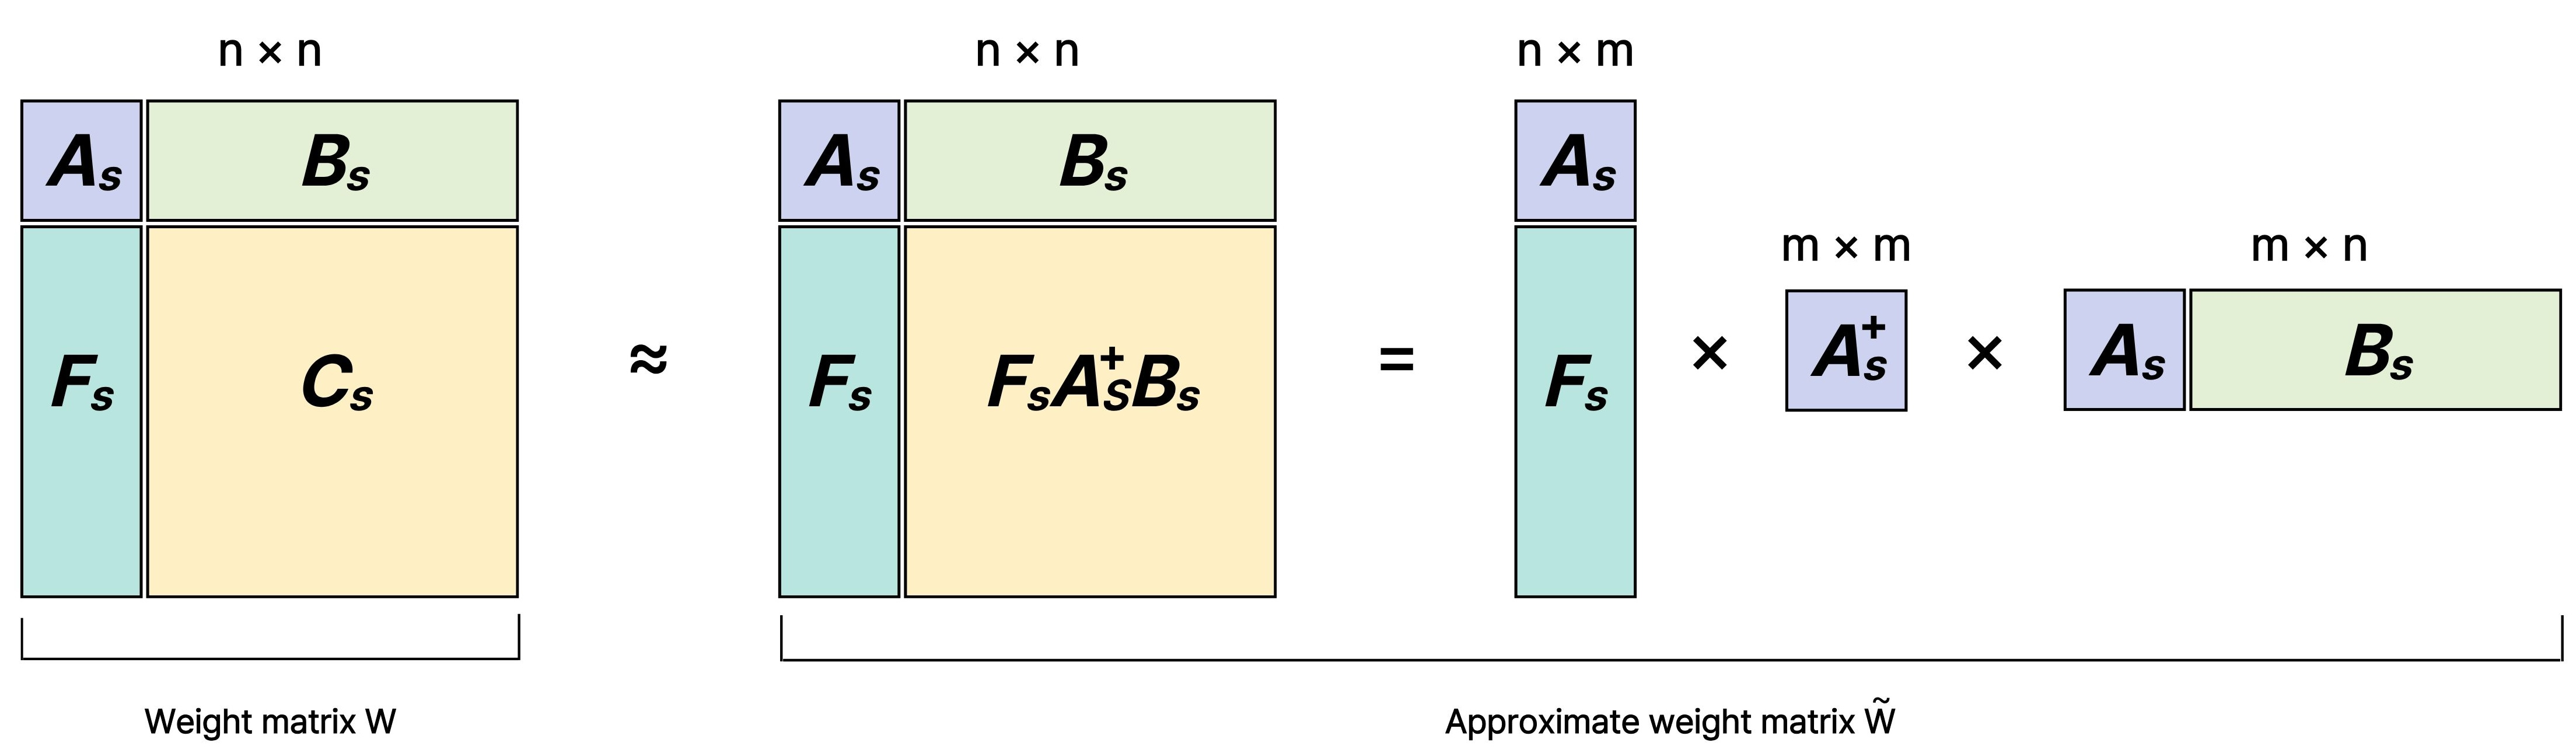
\includegraphics[width=0.49\textwidth]{../images/nystrom-approx.jpg}%
    }\quad
    \subfloat[Our \name{} Freivalds' Check\label{fig:zkdiet}]{%
        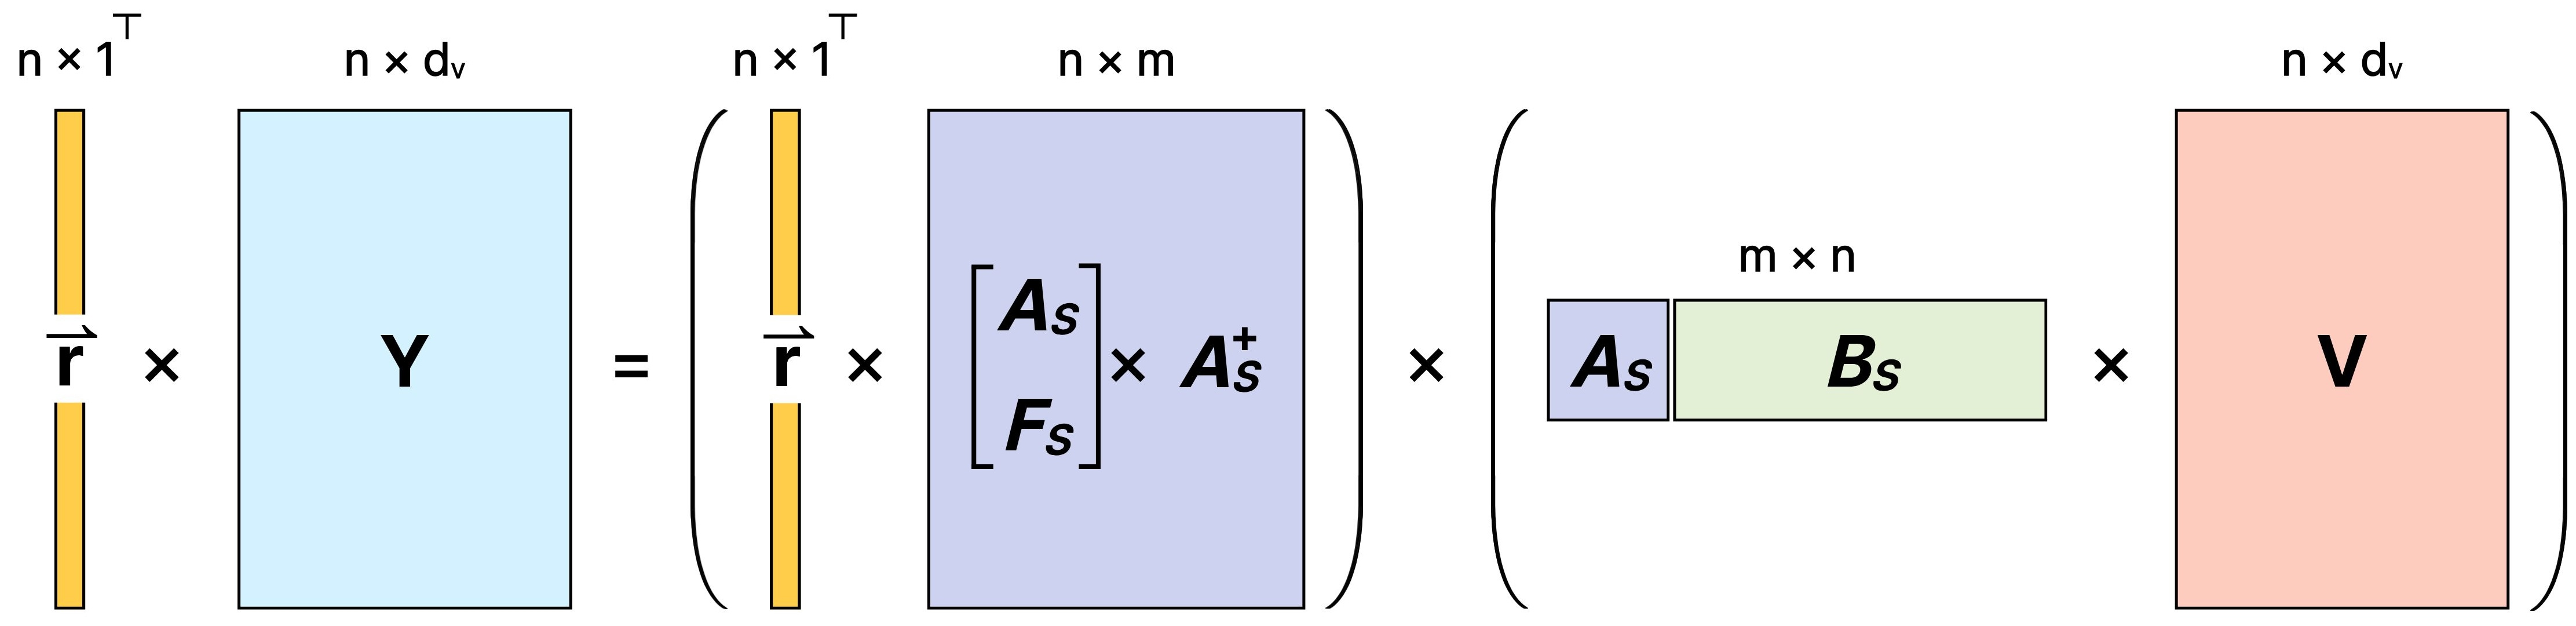
\includegraphics[width=0.49\textwidth]{../images/zkdiet-freivald.jpg}%
    }
    \caption{Low-rank matrix multiplication with Freivalds' algorithm}
\end{figure}

% 그림 1에서 보이듯이, 우리는 $n \times n$ 크기의 Self-attention 행렬을 직접 다루는 대신, 이를 $n \times m$, $m \times m$, $m \times n$ 형태의 저차원 행렬들로 분해하는 Nyströmformer의 절차를 수행한다. 이렇게 얻어진 Low-rank 표현에 대하여 Freivalds 알고리즘을 적용함으로써(그림 2), 검증 단계에서의 연산 부하를 $O(n^2)$에서 $O(mn)$ 수준인 $m(mn+d_v n)$ 크기의 벡터 곱으로 압축한다. 이를 통해 증명자(Prover)의 증명 생성 시간과 검증자(Verifier)의 오버헤드를 동시에 최소화할 수 있다.

As illustrated in Figure~\ref{fig:nystrom-approx}, rather than directly handling the $n \times n$ self-attention matrix, we follow the Nyströmformer procedure and decompose it into a sequence of low-dimensional matrices of shapes $n \times m$, $m \times m$, and $m \times n$. we denote the three low-rank factors by
$\tilde{F} := \mathrm{softmax}(Q\tilde{K}^{\top}/\sqrt{d_k}) \in \mathbb{F}^{n \times m}$,
$\tilde{A} := \mathrm{softmax}(\tilde{Q}\tilde{K}^{\top}/\sqrt{d_k}) \in \mathbb{F}^{m \times m}$, and
$\tilde{B} := \mathrm{softmax}(\tilde{Q}K^{\top}/\sqrt{d_k}) \in \mathbb{F}^{m \times n}$,
treated formally in Section~\ref{subsec:nystrom-attention}.
In the block decomposition of Figure~\ref{fig:nystrom-approx}, $\tilde{F}$, $\tilde{A}^{+}$, and
$\tilde{B}$ take the roles of
$\bigl[\begin{smallmatrix} A_S \\ F_S \end{smallmatrix}\bigr]$,
$A_S^{+}$, and $\bigl[\, A_S \;\; B_S \,\bigr]$, respectively;
they are computed from the landmarks before the softmax rather than
extracted from $S$ (cf.\ Section~\ref{subsec:nystrom-linear}), so Figure~\ref{fig:zkdiet} is obtained from
Figure~\ref{fig:nystrom-approx} by this substitution. By applying Freivalds’ algorithm to this low-rank representation (Figure~\ref{fig:zkdiet}), we compress the verification workload from $O(n^2)$ to $O(n)$, effectively reducing it to a chain of vector--matrix products of total size $2nm + m^2 + nd_v$: multiplying the random vector by $\tilde{F}$ ($nm$), then by $\tilde{A}^{+}$ ($m^2$), then by $\tilde{B}$ ($mn$), and finally by~$\V$ ($nd_v$). The pseudoinverse factor is instantiated by the iterative approximation $Z^{*}$ of Section~\ref{subsec:nystrom-linear}: the prover computes $Z^{*}$ outside the circuit and supplies it as a witness, and our protocol verifies in-circuit that $Z^{*}$ satisfies the Moore--Penrose conditions (Section~\ref{moore-penrose}) up to quantization tolerance. Since these conditions uniquely characterize the pseudoinverse $\tilde{A}^{+}$, this check constrains $Z^{*}$ to a small neighborhood of $\tilde{A}^{+}$, without ever computing $\tilde{A}^{+}$ itself.

% 이처럼 축소된 행렬곱을 Freivalds 알고리즘에 기반하여 검증하기 위해, 우리는 Commit-and-Prove SNARK (CP-SNARK) 구조를 채택한다. 먼저 어텐션 행렬은 회로 외부에서 커밋되고, 증명자는 커밋된 행렬이 회로 내부의 비공개 증인(witness)과 일관됨을 보이는 동시에, low-rank 근사 연산으로 얻어진 행렬곱 결과가 올바름을 저차원 근사에 최적화된  선형 복잡도의 Freivalds 검증을 통해 증명한다. 전체 어텐션 행렬 대신 외부에서 생성된 커밋먼트(commitment)만을 검증자에게 전달함으로써, 검증자는 상수 시간의 커밋 검증만 수행하면 된다. 이러한 설계는 대규모 모델에서 발생하는 행렬 연산에 대해, 증명 생성 비용과 검증 비용을 동시에 크게 감소시킨다.
% 영지식 회로는 유한체 위에서 동작하기 때문에, 실수 기반 Transformer 연산을 그대로 표현할 수 없다. 따라서 우리는 연산을 정밀도 손실을 최소화하는 방식으로 양자화하였으며, 이 과정에서 ZEN~\cite{…}에서 제안된 R1CS friendly quantization technique을 사용하였다.

\begin{figure*}[!ht]
    \centering
    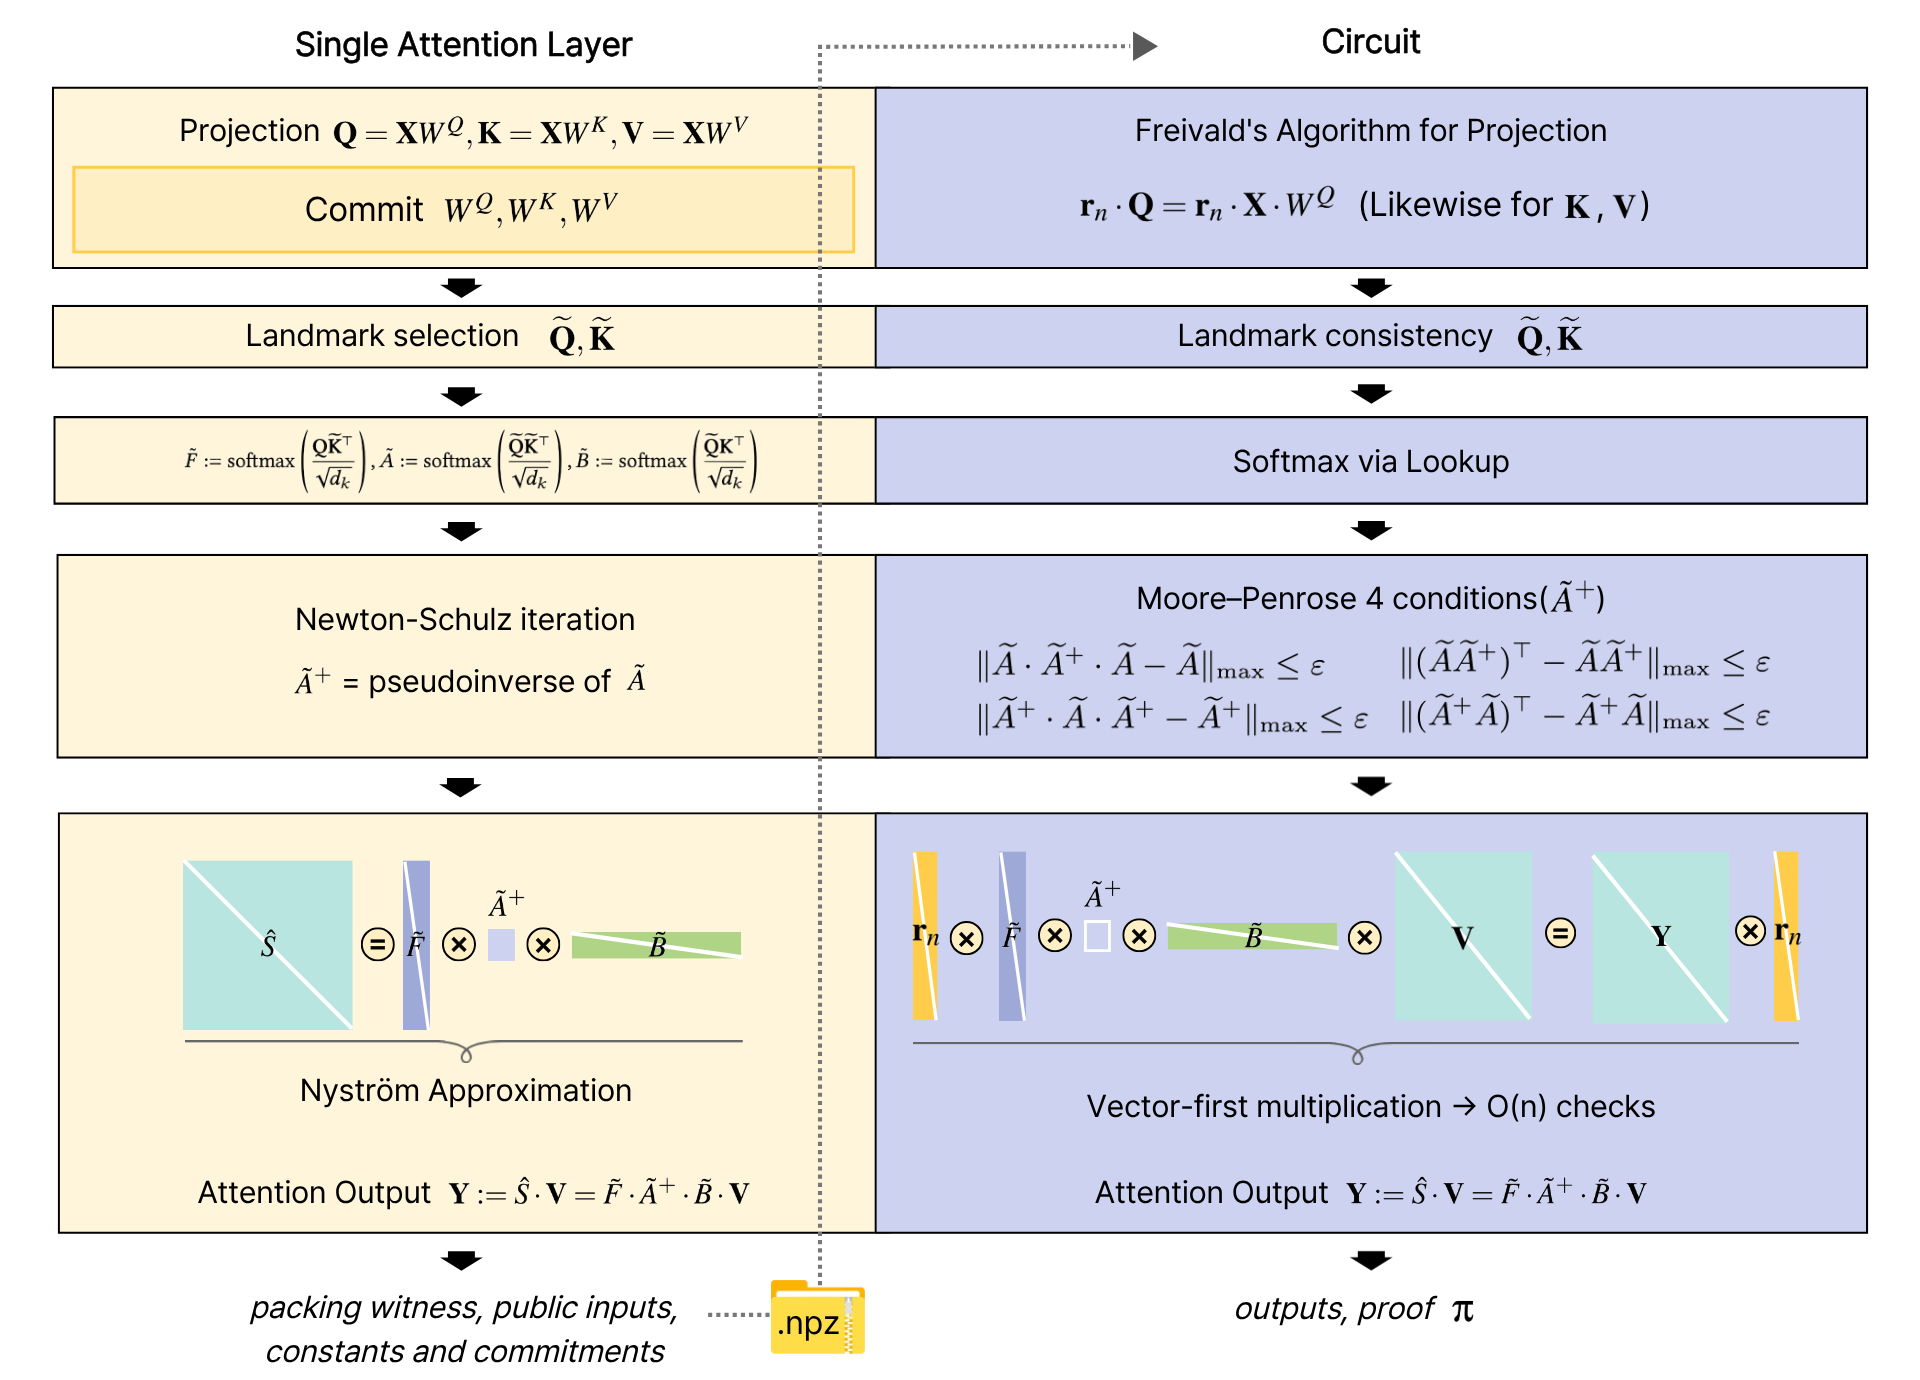
\includegraphics[width=0.6\linewidth]{../images/overview.png}
    \caption{Overview of Self-Attention and our framework}
    \label{fig:attention-overview}
\end{figure*}

To verify such low-rank matrix multiplications using Freivalds' algorithm, we adopt a commit-carrying SNARK (CC-SNARK) architecture (Figure~2). To ensure that a fixed model is persistently used across multiple user queries, the model weight matrices $W_Q, W_K, W_V, W_O$ are initially committed using a relation-independent key to establish a published global weight commitment ($c_W$). During execution, the CC-SNARK circuit extracts its own relation-dependent weight commitments ($cm_W^i$), and the prover demonstrates via $CP_{\mathrm{link}}$ that these internal commitments correspond to the same weights in $c_W$, while simultaneously proving the matrix multiplication result via Freivalds' algorithm with linear complexity. Instead of transmitting the full weight matrices, only the commitments are provided to the verifier, who then performs merely constant-time commitment checks. This design substantially reduces both proving and verification costs for matrix operations arising in large-scale models.
Because zero-knowledge circuits operate over finite fields, real-valued Transformer computations cannot be represented directly. We therefore quantize the computations in a manner that minimizes precision loss, leveraging the R1CS-friendly quantization technique proposed in~\cite{ZEN}. From this point onward, all matrices are understood to be over the finite field $\mathbb{F}$ after quantization.

%To verify such low-rank matrix multiplications using Freivalds' algorithm, we adopt a unified Commit-and-Prove architecture that integrates a commit-carrying backend ($\Pi_{cc}$) with CP-linkage (Figure~\ref{fig:protocol}). First, the model weight matrices $W = (W^i)_{i \in \{Q,K,V,O\}}$ are first committed outside the circuit as a long-lived commitment $c_W$. During query execution, the prover generates per-proof commitments $\widetilde{\cm}_{W^i}$ and $\widetilde{\cm}_{\mathsf{lk}}$, and constructs a single composite proof $\pi \gets \Pi_{\mathsf{zkdiet}}.\mathsf{prove}(\dots)$. This proof simultaneously asserts: (i)~the consistency between the long-lived commitment $c_W$ and the circuit-bound weight witnesses via weight CP-linkage,
%(ii)~the consistency between the non-linear intermediate values used in the main circuit and those bound to the lookup argument via operand CP-linkage,
%(iii)~the validity of the non-linear function evaluations asserting that these intermediate values correctly reside in the lookup table, and
%(iv)~the integrity of the low-rank matrix evaluations via Freivalds' algorithm in linear time.

%By supplying only the externally generated commitments and the unified proof $\pi$ to the verifier, the in-circuit setup and verification overhead for large public weight vectors are reduced to constant-time group operations. This design substantially reduces both proving and verification costs for matrix operations arising in Transformer-scale models.

%Because zero-knowledge circuits operate over finite fields, real-valued Transformer computations cannot be represented directly. We therefore quantize all computations to minimize precision loss, leveraging the R1CS-friendly quantization technique proposed in~\cite{ZEN}. From this point onward, all matrices and vectors are understood to be evaluated over the finite field $\mathbb{F}$ after quantization.

\begin{figure*}[!ht]
\center
\fbox{\procedure[head=\textbf{Protocol}, bodylinesep=2mm]{}{
        \mathcal{P}(\ck, c_W, \X; \{ W^Q, W^K, W^V, W^O\}) \< \< \mathcal{V}(\vk, c_W, \X) \\
        (\Y', \textit{aux}, \mathsf{lk}) \gets \NystromAttention(\X, W^Q, W^K, W^V, W^O) \\
        \widetilde{\cm}_{W^i} \gets \Com.\commit(\ck,W^i;\tilde{o}_i) \text{ for } i \in \{Q,K,V,O\} \\
        \widetilde{\cm} \gets \Com.\commit(\ck, \mathsf{lk} ;\tilde{o}) \\
        \<  \sendmessageright*[2cm]{\{\widetilde{\cm}_{W^i}\}_{i \in \{Q,K,V,O\}}, \widetilde{\cm}, \Y'\;} \< \\
        \< \sendmessageleft*[2cm]{\rand_n, \rand_m } \< \rand_n \sample \F^n, \t \rand_m \sample \F^m  \\
        \ins := \{ \X, \Y', \rand_n, \rand_m \} \\
        \comwit := \{ (W^i,\tilde{o}_i)_{i \in \{Q,K,V,O\}}, (\mathsf{lk}, \tilde{o}), (W^i,o_i)_{i \in \{Q,K,V,O\}} \} \\
        \uncomwit := \textit{aux} \\
        \pi \gets \Pi_\mathsf{zkdiet}.\prove( \pk, \ins; (\comwit, \uncomwit)) \\
        \<  \sendmessageright*[2cm]\pi \< \\
        \< \< \Pi_\mathsf{zkdiet}.\verify(\vk, \ins, \{\widetilde{\cm}_{W^i}\}_{i \in \{Q,K,V,O\}},\, \widetilde{\cm}, c_W, \pi)
    }}
    \caption{Our protocol}
    \label{fig:protocol}
\end{figure*}

%-------------------------------------------------------------------------------
\section{\name: Efficient Proofs of Low-Rank Matrix Multiplication via Freivalds' Algorithm}
\label{sec:protocol}
%-------------------------------------------------------------------------------

In this section, we present the core protocol of \name. Our goal is to prove the correctness of \nystrom-approximated low-rank self-attention while avoiding any explicit computation of the $n \times n$ attention matrix inside the circuit. Concretely, we design the protocol so that the number of constraints scales linearly with the sequence length $n$. To this end, we adopt a commit-carrying SNARK (CC-SNARK) architecture that pushes computationally expensive operations (e.g., large matrix multiplications and pseudoinverse computation) outside the circuit, and proves only their correctness inside the circuit using a small number of constraints.


\subsection{Protocol Overview}
Our protocol follows the message flow shown in Figure~\ref{fig:protocol}.
Prior to answering any query, the model provider generates a long-lived global commitment $c_W \gets \Com.\commit(\ck_{\mathrm{glob}}, W; o)$ to its weight matrices $W = (W^Q, W^K, W^V, W^O)$ under randomness $o$ using the circuit-independent key $\ck_{\mathrm{glob}}$, and publishes $c_W$ once to bind all future inferences to this specific model.

When a query arrives, the prover $\mathcal{P}$ first executes $\NystromAttention$ locally outside the circuit on the input sequence $\X \in \mathbb{F}^{n \times d}$ and the weight matrices $W$.
From this local evaluation, the prover obtains the final attention output $\Y'$, the non-linear intermediate operands $\mathsf{lk} := (\tilde{F}, \tilde{A}, \tilde{B})$, and the auxiliary intermediate matrices $\textit{aux}$.

Next, the prover commits to the weight matrices $W^Q, W^K, W^V, W^O$ under the circuit-dependent key $\ck$, producing $\widetilde{\cm}_{W^i} = \Com.\commit(\ck, W^i; \tilde{o}_i)$ for $i \in \{Q,K,V,O\}$.
The prover also commits to the non-linear operands $\mathsf{lk}$, yielding the proof-dependent commitment $\widetilde{\cm} = \Com.\commit(\ck, \mathsf{lk}; \tilde{o})$.
The prover then transmits the weight commitments $\{\widetilde{\cm}_{W^i}\}_{i \in \{Q,K,V,O\}}$, the commitment $\widetilde{\cm}$, and the plaintext output $\Y'$ to the verifier $\mathcal{V}$.
In response, the verifier samples random challenge vectors $\rand_n \sample \mathbb{F}^n$ and $\rand_m \sample \mathbb{F}^m$ for Freivalds' randomized checks and sends them back to the prover.

The public instance for the proof system is established as
\[
    \ins := (\X, \Y', \rand_n, \rand_m).
\]
The witness is organized into two primary categories: committed witnesses ($\comwit$) and uncommitted witnesses ($\uncomwit$).
The committed part,
\[
    \comwit := \{ (W^i,\tilde{o}_i)_{i \in \{Q,K,V,O\}}, (\mathsf{lk}, \tilde{o}), (W^i,o_i)_{i \in \{Q,K,V,O\}} \},
\]
is bound by the local weight commitments $\{\widetilde{\cm}_{W^i}\}$ and the non-linear commitment $\widetilde{\cm}$, alongside the randomness $o$ of the global commitment $c_W$.
The uncommitted witness consists of the remaining intermediate matrices, $\uncomwit := \textit{aux}$, where the full auxiliary tuple is explicitly defined as
\[
    \textit{aux} := \bigl(\Q, \K, \V,\; \widetilde{\Q}, \widetilde{\K},\; \Q\widetilde{\K}^{\top},\; \widetilde{\Q}\widetilde{\K}^{\top},\; \widetilde{\Q}\K^{\top},\; \tilde{F}, \tilde{A}, \tilde{B},\; \tilde{A}^{+},\; \Y\bigr).
\]
Although these witness intermediates carry no direct commitment, they cannot be manipulated by a malicious prover: each intermediate matrix is strictly constrained by the chain of circuit equalities (and Freivalds' checks) that bridge the committed weights on one end, the committed non-linear operands $\mathsf{lk}$ in the middle, and the public output $\Y'$ on the other.
Because all committed values---both weight commitments and $\widetilde{\cm}$---are fixed prior to sampling the challenges $\rand_n, \rand_m$, the soundness of the Freivalds randomized verification is preserved.

For notational simplicity, we write $\tilde{A}^{+}$ for the corresponding pseudoinverse of $\tilde{A}$ throughout this section, with the understanding that the value actually supplied is the iterative approximation $Z^{*}$ of Section~\ref{subsec:nystrom-linear}, and that the Moore--Penrose checks of Section~\ref{moore-penrose}, verified up to quantization tolerance, are what license this identification.

Finally, the prover invokes the unified proof system to generate a composite proof $\pi \gets \Pi_{\mathsf{zkdiet}}.\prove(\pk, \ins; (\comwit, \uncomwit))$ and transmits $\pi$ to the verifier.
This unified proof $\pi$ encapsulates the commit-carrying proof alongside two CP-linkages that bind $\{\widetilde{\cm}_{W^i}\}$ to the long-lived global commitment $c_W$ and $\widetilde{\cm}$ to the lookup arguments.
The verifier then checks the proof via $\Pi_{\mathsf{zkdiet}}.\verify(\vk, \ins, \{\widetilde{\cm}_{W^i}\}_{i \in \{Q,K,V,O\}},\, \widetilde{\cm}, c_W, \pi)$.
In the non-interactive variant, the challenges $\rand_n, \rand_m$ are derived via the Fiat--Shamir transformation from the transcript $(\X, \Y', \{\widetilde{\cm}_{W^i}\}_{i \in \{Q,K,V,O\}}, \widetilde{\cm}, c_W)$, ensuring that all commitments are bound before challenge generation.
%Our protocol follows the message flow shown in Figure~\ref{fig:protocol}.
%First, the prover $\mathcal{P}$ executes $\NystromAttention$ locally outside the circuit on the input sequence $\X \in \mathbb{F}^{n \times d}$ and the %weight matrices $W^Q, W^K, W^V, W^O \in \mathbb{F}^{d \times d}$.
%Because this execution is performed off-circuit, it can seamlessly accommodate heavy intermediate operations such as the Moore--Penrose pseudoinverse computation.
%From this local evaluation, the prover obtains the final attention output $\Y'$, the non-linear intermediate operands $\mathsf{lk} := (\tilde{F}, \tilde{A}, \tilde{B})$, and the auxiliary intermediate matrices $\textit{aux}$.

%Next, the prover commits to the weight matrices $W^Q, W^K, W^V, W^O$, producing $\widetilde{\cm}_{W^i} = \Com.\commit(\ck, W^i; \tilde{o}_i)$ for $i \in \{Q,K,V,O\}$.
%The prover also commits to the non-linear operands $\mathsf{lk}$, yielding the proof-dependent commitment $\widetilde{\cm} = \Com.\commit(\ck, \mathsf{lk}; \tilde{o})$.
%The prover then transmits the weight commitments $\{\widetilde{\cm}_{W^i}\}_{i \in \{Q,K,V,O\}}$, the commitment $\widetilde{\cm}$, and the plaintext output $\Y'$ to the verifier $\mathcal{V}$.
%In response, the verifier samples random challenge vectors $\rand_n \sample \mathbb{F}^n$ and $\rand_m \sample \mathbb{F}^m$ for Freivalds' randomized checks and sends them back to the prover.

%The public instance for the proof system is established as
%\[
%    \ins := (\X, \Y', \rand_n, \rand_m).
%\]
%The witness is organized into two primary categories: committed witnesses ($\comwit$) and uncommitted witnesses ($\uncomwit$).
%The committed part,
%\[
%    \comwit := \left(\{ (W^i, \tilde{o}_i) \}_{i \in \{Q,K,V,O\}}, (\mathsf{lk}, \tilde{o})\right),
%\]
%is bound by the weight commitments $\{\widetilde{\cm}_{W^i}\}$ and the non-linear commitment $\widetilde{\cm}$. The commitment $\widetilde{\cm}$ serves as the anchor for the CP-link with the lookup arguments for non-linear operations.
%The uncommitted witness consists of the remaining intermediate matrices, $\uncomwit := \textit{aux}$, where the full auxiliary tuple is explicitly defined as
%\[
%    \textit{aux} := \bigl(\Q, \K, \V,\; \widetilde{\Q}, \widetilde{\K},\; \Q\widetilde{\K}^{\top},\; \widetilde{\Q}\widetilde{\K}^{\top},\; \widetilde{\Q}\K^{\top},\; \tilde{F}, \tilde{A}, \tilde{B},\; \tilde{A}^{+},\; \Y\bigr).
%\]
%Although these witness intermediates carry no direct commitment, they cannot be manipulated by a malicious prover: each intermediate matrix is strictly constrained by the chain of circuit equalities (and Freivalds' checks) that bridge the committed weights on one end, the committed non-linear operands $\mathsf{lk}$ in the middle, and the public output $\Y'$ on the other.
%Because all committed values---both weight commitments and $\widetilde{\cm}$---are fixed prior to sampling the challenges $\rand_n, \rand_m$, the soundness of the Freivalds randomized verification is preserved.

%For notational simplicity, we write $\tilde{A}^{+}$ for the corresponding witness slot throughout this section, with the understanding that the value actually supplied is the iterative approximation $Z^{\star}$ of Section~\ref{subsec:nystrom-linear}, and that the Moore--Penrose checks of Section~\ref{moore-penrose}, verified up to quantization tolerance, are what license this identification.

%Finally, the prover generates the SNARK proof $\pi \gets \Pi_\cc.\prove(\pk, \ins; (\comwit, \uncomwit))$ and transmits $\pi$ to the verifier.
%The verifier then checks the proof via $\Pi_\cc.\verify(\vk, \ins, \{\widetilde{\cm}_{W^i}\}_{i \in \{Q,K,V,O\}},\, \widetilde{\cm}, \pi)$.
%In the non-interactive variant, the challenges $\rand_n, \rand_m$ are derived via the Fiat--Shamir transformation from the transcript $(\X, \Y', \{\widetilde{\cm}_{W^i}\}_{i \in \{Q,K,V,O\}}, \widetilde{\cm})$, ensuring that all commitments are bound before the challenge generation.


% \begin{algorithm}[h]
% \raggedright
% \scalebox{1}{
% \small
% \begin{minipage}{0.95\linewidth}
% \textbf{Input: } \text{model parameters } $W^Q, W^K, W^V \in \mathbb{F}^{d \times d}$ \\
% \textbf{Output: } commitments $\cm_Q, \cm_K, \cm_V$ \\[2pt]
% \underline{$\comparams(W^Q, W^K, W^V)$}: \\[2pt]
% \pseudocode[colspace,linenumbering]{
%   o_Q, o_K, o_V \sample \mathbb{F} \\
%   \cm_Q \gets \ped.\commit(\ck, W^Q; o_Q) \\
%   \cm_K \gets \ped.\commit(\ck, W^K; o_K) \\
%   \cm_V \gets \ped.\commit(\ck, W^V; o_V) \\
%   \pcreturn (\cm_Q, \cm_K, \cm_V)
% }
% \end{minipage}
% }
% \caption{Commit model parameters}
% \label{algo:commit}
% \end{algorithm}

\subsection{\nystrom-Based Low-Rank Self-Attention}\label{subsec:nystrom-attention}
Our system adopts a \nystrom-based low-rank approximation for self-attention. In \nystromformer, the query and key matrices are represented using $m$ landmark vectors.
Algorithm~\ref{alg:landmark} describes the landmark selection procedure. Given $\Q=[\mathbf{q}_1,\ldots,\mathbf{q}_n]^\top$ and $\K=[\mathbf{k}_1,\ldots,\mathbf{k}_n]^\top$, we summarize the length-$n$ sequence using $m$ landmarks by partitioning it into $m$ consecutive segments of length $\ell = n/m$ and defining each landmark as the average over the $\ell$ tokens in its segment. This yields $\widetilde{\Q}=[\tilde{\mathbf{q}}_1,\ldots,\tilde{\mathbf{q}}_m]^\top$ and $\widetilde{\K}=[\tilde{\mathbf{k}}_1,\ldots,\tilde{\mathbf{k}}_m]^\top$.
With these landmarks, we avoid constructing the full $n\times n$ attention matrix and instead decompose the computation into three lower-dimensional matrices: $\Q\widetilde{\K}^{\top} \in \mathbb{F}^{n \times m}, \widetilde{\Q}\widetilde{\K}^{\top} \in \mathbb{F}^{m \times m}, \widetilde{\Q}\K^{\top} \in \mathbb{F}^{m \times n}$
% an $n\times m$ matrix $\Q\widetilde{\K}^{\top}$, a $m\times m$ matrix $\widetilde{\Q}\widetilde{\K}^{\top}$, and a $m\times n$ matrix $\widetilde{\Q}\K^{\top}$.

We then apply the row-wise softmax to each of these matrices and compute
\[
\tilde{F} := \sfmax\!\Bigl(\tfrac{\Q\widetilde{\K}^{\top}}{\sqrt{d_k}}\Bigr),
\tilde{A} := \sfmax\!\Bigl(\tfrac{\widetilde{\Q}\widetilde{\K}^{\top}}{\sqrt{d_k}}\Bigr),
\tilde{B} := \sfmax\!\Bigl(\tfrac{\widetilde{\Q}\K^{\top}}{\sqrt{d_k}}\Bigr).
\]
Here, $\tilde{A}$ is a small $m\times m$ matrix corresponding to the landmark submatrix of the original $n \times n$ attention matrix.
Overall, the combination of $\tilde{F}$, $\tilde{A}$, and $\tilde{B}$ yields a \nystrom\ approximation of the full attention map.

Finally, we compute an approximation to the Moore--Penrose pseudoinverse $\tilde{A}^{+}$ of the $m\times m$ matrix $\tilde{A}$. While one could compute $\tilde{A}^{+}$ via SVD, this is typically inefficient on GPU hardware. Therefore, \nystromformer\ approximates $\tilde{A}^{+}$ via an iterative polynomial approximation to the SVD. Algorithm~\ref{alg:inverse} shows this iterative procedure. 

Using the resulting $\tilde{A}^{+}$, we form the final approximated attention matrix
\[
    \hat{S} := \tilde{F}\cdot \tilde{A}^{+}\cdot \tilde{B},
\]
and compute the attention output as
\[
    \Y := \hat{S} \cdot \V.
\]
Finally, the output projection is applied using the weight matrix $\W^O \in \mathbb{F}^{d \times d}$:
\[
    \Y' := \Y \cdot \W^O.
\]
Algorithm~\ref{alg:nystromAttention} provides the complete \nystrom-based self-attention computation used in our framework.

\begin{algorithm}[t!]
    \raggedright
    \small
    \begin{minipage}{0.95\linewidth}
    \textbf{Input: } Query $\Q$, Key $\K \in \F^{n \times d}$;
    number of landmarks $m$ with $m \mid n$ \\
    \textbf{Output: } Landmark matrices $\widetilde{\Q}, \widetilde{\K} \in \F^{m \times d}$ \\[2pt]
    \underline{$\selectLandmarks(\Q, \K, m)$:}\\[2pt]
    \pseudocode[colspace,linenumbering]{
        \pcparse \Q = [\mathbf{q}_1; \dots; \mathbf{q}_n]^\top,\;
                 \K = [\mathbf{k}_1; \dots; \mathbf{k}_n]^\top
                 \text{ (rows } \mathbf{q}_i, \mathbf{k}_i \in \F^d) \\
        \ell \gets n / m \\
        \pcfor j \in \{1, \dots, m\} \pcdo \\
            \t \tilde{\mathbf{q}}_j \gets \frac{1}{\ell}
                \sum_{i=(j-1)\ell + 1}^{j\ell} \mathbf{q}_i, \quad
                \tilde{\mathbf{k}}_j \gets \frac{1}{\ell}
                \sum_{i=(j-1)\ell + 1}^{j\ell} \mathbf{k}_i \\
        \pcendfor \\
        \widetilde{\Q} \gets [\tilde{\mathbf{q}}_1; \dots; \tilde{\mathbf{q}}_m]^\top,\;
        \widetilde{\K} \gets [\tilde{\mathbf{k}}_1; \dots; \tilde{\mathbf{k}}_m]^\top \\
        \pcreturn (\widetilde{\Q}, \widetilde{\K})
    }
    \end{minipage}
    \caption{Select landmarks}
    \label{alg:landmark}
\end{algorithm}

\begin{algorithm}[t!]
\raggedright
\scalebox{1}{
\small
\begin{minipage}{0.95\linewidth}
\textbf{Input: } $\text{selected landmark matrix } \tilde{A} \in \mathbb{F}^{m \times m}$\\
\textbf{Output: } $\text{approximate pseudoinverse }\tilde{A}^+ \in \mathbb{F}^{m \times m}$\\[2pt]
\underline{$\computeMPInverse(\tilde{A})$}: \\[2pt]
\pseudocode[colspace,linenumbering]{
  Z_0 \gets \tilde{A}^\top / \left(\|\tilde{A}\|_1 \cdot \|\tilde{A}\|_\infty\right) \\
  \text{Set } T \text{ (e.g., } T=6 \text{ iterations)} \\
  \pcfor t \in \{0,\dots,T-1\} \pcdo \\
    \t Z_{t+1} \gets \frac{1}{4} Z_t \Big( 13I - \tilde{A}Z_t\big(15I - \tilde{A}Z_t(7I - \tilde{A}Z_t)\big) \Big) \\
  \pcendfor \\
  \tilde{A}^+ \gets Z_T \\
  \pcreturn \tilde{A}^+
}
\end{minipage}
}
\caption{Compute Moore--Penrose inverse}
\label{alg:inverse}
\end{algorithm}


\begin{algorithm}[!t]
    \raggedright
    \scalebox{1}{
    \small
    \begin{minipage}{0.95\linewidth}
    \noindent
    \begin{tabular}{@{}l l@{}}
    \textbf{Input:} & \text{Input sequence } $\X \in \mathbb{F}^{n \times d}$, \\
    & \text{Model parameters } $W^Q, W^K, W^V, W^O \in \mathbb{F}^{d \times d}$ \\[3pt]
    \textbf{Output:} & \text{Attention output } $\Y' \in \mathbb{F}^{n \times d}$, \\
    & \text{Auxiliary intermediates } $\textit{aux}$, \\
    & \text{Non-linear operands } $\mathsf{lk} := (\tilde{F}, \tilde{A}, \tilde{B})$ \\ [2pt]
    \end{tabular}
    
    \underline{$\NystromAttention(\X, W^Q, W^K, W^V, W^O)$}: \\[2pt]
    $%
    \pseudocode[colspace,linenumbering]{
        \Q := \X W^Q, \quad \K := \X W^K, \quad \V := \X W^V \\[2pt]
        \widetilde{\Q}, \widetilde{\K} \gets \selectLandmarks(\Q, \K) \\[2pt]
        \tilde{F} := \sfmax\left(\frac{\Q\widetilde{\K}^\top}{\sqrt{d_k}}\right), \quad \tilde{A} := \sfmax\left( \frac{\widetilde{\Q}\widetilde{\K}^\top}{\sqrt{d_k}} \right), \quad \tilde{B} := \sfmax\left(\frac{\widetilde{\Q}\K^\top}{\sqrt{d_k}}\right) \\[2pt]
        \tilde{A}^+ \gets \computeMPInverse(\tilde{A}) \\[2pt]
        \Y := (\tilde{F} \cdot \tilde{A}^+) (\tilde{B} \cdot \V) \\[2pt]
        \Y' := \Y \cdot W^O \\[2pt]
        \textit{aux} := (\Q, \K, \V, \widetilde{\Q}, \widetilde{\K}, \Q\widetilde{\K}^\top, \widetilde{\Q}\widetilde{\K}^\top, \widetilde{\Q}\K^\top, \tilde{A}^+, \Y) \\[2pt]
        \mathsf{lk} := (\tilde{F}, \tilde{A}, \tilde{B}) \\[2pt]
        \pcreturn (\Y', \textit{aux}, \mathsf{lk})
    }%
    $
    \end{minipage}
    }
    \caption{\nystrom\ approximation of attention matrix}
    \label{alg:nystromAttention}
\end{algorithm}

\subsection{Efficient Verification via Freivalds’ Algorithm}
\label{moore-penrose}
Our protocol uses Freivalds’ algorithm as a core tool to efficiently verify that the low-rank self-attention computation is performed correctly. In particular, within the zk-SNARK circuit, we employ Freivalds’ algorithm to ensure that the following key operations can be verified with linear cost. \\

\sss{Query/Key/Value matrix generation and output projection}
Using the verifier's random vector $\rand_n$, we check the relation $\Q = \X \W^Q$ by comparing $\rand_n^{\top} \Q$ with $\rand_n^{\top}(\X \W^Q)$.
We verify $\K$ and $\V$ in the same way. Rather than proving the full $n\times d$ matrix product directly, this Freivalds' check reduces verification to computing only the vector-matrix product $\rand_n^{\top}\X W^Q$, thereby reducing the complexity from $\mathcal{O}(n d^2)$ to $\mathcal{O}(nd + d^2)$. The output projection $\Y'=\Y \W^O$ is verified analogously: we check $\rand_n^{\top}\Y' \stackrel{?}{=} (\rand_n^{\top}\Y)\,W^O$. \\

\sss{Low-rank matrix operations}
We also verify low-dimensional products such as $\Q\widetilde{\K}^{\top}$,
$\widetilde{\Q}\widetilde{\K}^{\top}$, and $\widetilde{\Q}\K^{\top}$
by multiplying each matrix with a random vector of matching dimension,
i.e., $\rand_n$ or $\rand_m$.
For instance, we can certify the correctness of $\Q\widetilde{\K}^{\top}$ by checking the following equality:
\[
\rand_n^{\top}\!\bigl(\Q\widetilde{\K}^{\top}\bigr)
\stackrel{?}{=}
(\rand_n^{\top}\Q)\,\widetilde{\K}^{\top}
\]

Similarly, the products $\widetilde{\Q}\widetilde{\K}^{\top}$ and $\widetilde{\Q}\K^{\top}$ are validated with linear cost, without explicitly computing the full matrix multiplications inside the circuit. \\

\sss{Moore--Penrose pseudoinverse}
As shown in Algorithm~\ref{alg:inverse},computing the Moore--Penrose pseudoinverse $\tilde{A}^{+}$ inside the circuit is inefficient.
Instead, the circuit certifies that the supplied matrix $\tilde{A}^{+}$ satisfies the four Moore--Penrose conditions, which correspond to lines~19--22 in Figure~\ref{fig:relation}.
Since $\tilde{A}^{+}$ is obtained by a finite Newton--Schulz iteration, these conditions are enforced up to a bounded residual $\varepsilon$; we defer the concrete tolerance to Section~\ref{subsec:pseudoinverse}.
\begin{itemize}
    \item $\lVert\tilde{A}\cdot\tilde{A}^{+}\cdot\tilde{A}-\tilde{A}\rVert \leq \varepsilon$
    \item $\lVert\tilde{A}^{+}\cdot\tilde{A}\cdot\tilde{A}^{+}-\tilde{A}^{+}\rVert \leq \varepsilon$
    \item $\lVert(\tilde{A}\tilde{A}^{+})^{\top}-\tilde{A}\tilde{A}^{+}\rVert \leq \varepsilon$
    \item $\lVert(\tilde{A}^{+}\tilde{A})^{\top}-\tilde{A}^{+}\tilde{A}\rVert \leq \varepsilon$
\end{itemize}
This allows the prover to efficiently demonstrate that $\tilde{A}^{+}$ approximately satisfies the pseudoinverse conditions without explicitly computing it in-circuit.

The relations that the prover must satisfy are formalized in Figure~\ref{fig:relation} as the definition of the circuit relation. In particular, the relation $\R(\ins,\wit)$ takes the public instance $\ins=(\X,\rand_n,\rand_m)$ and the witness $\wit=(W^Q, W^K, W^V, W^O, \Q,\K,\V, \Q\widetilde{\K}^\top, \widetilde{\Q}\widetilde{\K}^\top, \widetilde{\Q}\K^\top, \widetilde{A}^+, \Y, \mathbf{O})$, and enforces all required equalities as well as the softmax computation. All key equalities are expressed in the form of products with the random vectors, accordingly, the circuit computes only vector inner products.


\begin{figure}[t!]
\center
\fbox{\procedure[
    head=\textbf{Relation},
    bodylinesep=2mm,
    linenumbering,
    mode=text
]{}{
        $\R(\ins, \wit): $\\[2pt]
        $\t \pcparse \ins = (\X, \rand_n, \rand_m, \Y'), \wit = (\comwit, \uncomwit)$ \\
        $\t \pcparse \comwit := \{ (W^i,\tilde{o}_i)_{i \in \{Q,K,V,O\}}, (\mathsf{lk}, \tilde{o}), (W^i,o_i)_{i \in \{Q,K,V,O\}} \}$ \\
        $\t \pcparse \uncomwit = aux$ \\
        $\t \pcparse \Q = [\mathbf{q}_1, \mathbf{q}_2, \dots, \mathbf{q}_n]^\top, \K = [\mathbf{k}_1, \mathbf{k}_2, \dots, \mathbf{k}_n]^\top$ \\
        $\t \rand_n^\top \cdot \Q = \rand_n^\top \cdot \X \cdot W^Q$ \\
        $\t \rand_n^\top \cdot \K = \rand_n^\top \cdot \X \cdot W^K$ \\
        $\t \rand_n^\top \cdot \V = \rand_n^\top \cdot \X \cdot W^V$ \\
        $\t \pcfor j \in \{ 1, \dots, m\} \pcdo$ \\
            $\t \t\tilde{\mathbf{q}}_j \gets \sum_{i=(j-1) \times \ell + 1}^{j\ell}  \frac{\mathbf{q}_i}{\ell},
            \tilde{\mathbf{k}}_j \gets \sum_{i=(j-1) \times \ell + 1}^{j\ell} \frac{\mathbf{k}_i}{\ell}$ \\
        $\t \pcendfor$ \\
        $\t \widetilde{\Q} \gets [\tilde{\mathbf{q}}_1, \dots, \tilde{\mathbf{q}}_m]^\top, \widetilde{\K} \gets [\tilde{\mathbf{k}}_1, \dots, \tilde{\mathbf{k}}_m]^\top$ \\
        $\t \rand_n^\top \cdot \Q\widetilde{\K}^\top = \rand_n^\top \cdot \Q \cdot \widetilde{\K}^\top$ \\
        $\t \rand_m^\top \cdot \widetilde{\Q}\widetilde{\K}^\top = \rand_m^\top \cdot \widetilde{\Q} \cdot \widetilde{\K}^\top$ \\
        $\t \rand_m^\top \cdot \widetilde{\Q}\K^\top = \rand_m^\top \cdot \widetilde{\Q} \cdot \K^\top$ \\
        $\t \widetilde{F} = \sfmax\left( \frac{\Q\widetilde{\K}^\top}{\sqrt{d_k}} \right)$ \\
        $\t \widetilde{A} = \sfmax\left( \frac{\widetilde{\Q}\widetilde{\K}^\top}{\sqrt{d_k}} \right)$ \\
        $\t \widetilde{B} = \sfmax\left( \frac{\widetilde{\Q}\K^\top}{\sqrt{d_k}} \right)$ \\
        $\t \lVert \rand_m^\top \cdot \widetilde{A} \cdot \widetilde{A}^+ \cdot \widetilde{A} - \rand_m^\top \cdot \widetilde{A} \rVert \leq \varepsilon$ \\
        $\t \lVert \rand_m^\top \cdot \widetilde{A}^+ \cdot \widetilde{A} \cdot \widetilde{A}^+ - \rand_m^\top \cdot \widetilde{A}^+ \rVert \leq \varepsilon$ \\
        $\t \lVert \rand_m^\top \cdot (\widetilde{A}\widetilde{A}^+)^\top - \rand_m^\top \cdot \widetilde{A}\widetilde{A}^+ \rVert \leq \varepsilon$ \\
        $\t \lVert \rand_m^\top \cdot (\widetilde{A}^+\widetilde{A})^\top - \rand_m^\top \cdot \widetilde{A}^+\widetilde{A} \rVert \leq \varepsilon$ \\
        $\t \rand_n^\top \cdot \Y = \rand_n^\top \cdot \widetilde{F} \cdot \widetilde{A}^+ \cdot \widetilde{B} \cdot \V$ \\
        $\t \rand_n^\top \cdot \Y' = \rand_n^\top \cdot \Y \cdot W^O$
}}
\caption{Relation of \name}
\label{fig:relation}
\end{figure}

%\subsection{Security Analysis}
%\label{subsec:security}
%
%\krev{%
%$\name$ inherits the security guarantees of its building blocks---LegoGroth16~\cite{Legosnark} (CC-SNARK), Lasso~\cite{Lasso} (lookup argument), and Freivalds' algorithm~\cite{Freivalds}---composed via the CP-link mechanism~\cite{Legosnark, Vectis}.
%We state the three standard properties informally and sketch why each holds.
%
%\sss{Completeness}
%If the prover honestly executes $\NystromAttention$ and produces valid witnesses, the verifier always accepts.
%Every Freivalds check is an exact algebraic identity when the matrices are computed correctly, so the check passes with probability~1.
%The softmax and activation lookups are verified by Lasso against a precomputed table, which always accepts a correct evaluation.
%The three Moore--Penrose conditions enforced by the circuit (Section~\ref{moore-penrose}) hold within the range-check bounds, as empirically verified in Section~\ref{subsec:pseudoinverse}.
%Completeness then follows from the completeness of LegoGroth16.
%
%\sss{Knowledge Soundness}
%A malicious prover cannot convince the verifier of an incorrect statement except with negligible probability, under the $q$-SDH assumption (LegoGroth16) and the binding property of the polynomial commitment (Lasso).
%The critical ordering guarantee is that all committed values---the weight commitments $\{\widetilde{\cm}_{W^i}\}$ and the proof-dependent commitment $\widetilde{\cm}$---are fixed before the Freivalds challenges $\rand_n, \rand_m$ are sampled (Figure~\ref{fig:protocol}).
%By Freivalds' algorithm, each matrix-multiplication check has soundness error at most $1/|\F|$.
%With $k$ independent Freivalds checks over the BLS12-381 scalar field ($|\F| \approx 2^{255}$), the total Freivalds error is at most $k/|\F|$, which is negligible.
%The CP-link ensures that the committed witnesses are consistent between the Groth16 circuit and the Lasso lookup argument; any inconsistency would violate the binding property of the underlying Pedersen commitment.
%Combining via a union bound, the overall knowledge-soundness error is $\negl(\lambda)$.
%
%\sss{Zero-Knowledge}
%The verifier observes only the public instance $\ins = (\X, \rand_n, \rand_m)$, the commitments $\{\widetilde{\cm}_{W^i}\}, \widetilde{\cm}$, and the proof~$\pi$.
%The commitments are computationally hiding under the discrete logarithm assumption, revealing nothing about the committed weights or intermediate values.
%The proof~$\pi$ is zero-knowledge by the simulation property of LegoGroth16: a PPT simulator can produce proofs indistinguishable from real proofs without access to the witness.
%In the non-interactive variant, the challenges are derived via the Fiat--Shamir transformation, and zero-knowledge is preserved in the random oracle model.
%}% end \krev


%-------------------------------------------------------------------------------
% BEGIN COMMENTED OUT: Section 6 Security
%-------------------------------------------------------------------------------
%\section{Security}
%\label{sec:figs}
%%-------------------------------------------------------------------------------
%% 해당 섹션에서, 우리는 zkDietFormer가 completeness와 security requirements를 만족함을 보일 것이다. zkDietFormer는 기반이 되는 CC-Groth16 프로토콜의 특성을 상속받아 완전성, 건전성, 그리고 영지식성을 보장한다.
%In this section, we show that zkDietFormer satisfies the completeness and security requirements. Since zkDietFormer is built upon the cc-Groth16 protocol, it inherits its guarantees of completeness, soundness, and zero-knowledge.
%\sss{Completeness}
%% 정직한 증명자가 Nystromformer 기반의 리니어 어텐션 연산을 충실히 수행하고 증명을 생성했다면, 검증자는 이를 항상 수용한다. 본 시스템에서 완전성 오류가 발생할 수 있는 지점은 룩업 테이블을 통한 비선형 연산(지수 함수)이다. 행렬 연산의 경우 프리발드 알고리즘은 수식이 올바를 때 항상 참을 반환한다. 룩업 테이블의 경우, 이론적으로 분모가 0이 될 가능성이 존재하나, zkDiet는 양자화 과정에서 zero-point 조정을 통해 모든 입력값을 양수 영역으로 매핑함으로써 분모가 0으로 근사되어 검증이 실패할 확률을 수학적으로 배제한다.
%If an honest prover correctly performs the Nyströmformer-based linear attention computation and generates a proof, then the verifier always accepts it. In our system, the only potential source of completeness error arises from nonlinear operations handled via lookup tables (i.e., exponentiation operations). For matrix operations, the Freivalds’ algorithm always returns true when the equation is correct. In the case of lookup tables, one may theoretically consider situations where the denominator becomes zero. However, $\scheme$ avoids this issue through quantization with zero-point adjustment, which maps all inputs into the positive domain. As a result, any scenario in which the denominator is approximated as zero is mathematically eliminated, preserving completeness.
%
%
%\sss{Soundness}
%% 어떤 malicious한 prover이더라도 부정확한 행렬값 결과에 대하여 negl한 확률을 제외하고 verifier를 속일 수 없다. 우리의 시스템은 두가지 중요한 시큐리티 특성을 만족한다. 첫번째로. 행렬곱 $AB=C$의 무결성은 프리발드 알고리즘에 의해 보장되며, $AB \neq C$임에도 불구하고 랜덤 벡터 $x$에 대해 $ABx = Cx$가 성립할 확률은 유한체 $\mathbb{F}$의 크기에 반비례하는 $O(1/|\mathbb{F}|)$로 극히 낮다.
%Even a malicious prover cannot convince the verifier of an incorrect matrix computation except with negligible probability. Our system satisfies two essential security properties.
%
%First, the integrity of the matrix multiplication $AB = C$ is guaranteed by Freivalds’ algorithm. When $AB \neq C$, the probability that a randomly chosen vector $r$ satisfies $ABx = C$ is extremely small, bounded by $O(1/|\mathbb{F}|)$, which is inversely proportional to the size of the finite field $\mathbb{F}$. To simplify the analysis, we assume in the following proof that the random vector $r$ used in Freivalds’ algorithm is sampled from the binary domain $\{0,1\}^n$.
%%%%%%
%\begin{proof}
%% notation 수정 버전
%Since $\hat{D}^{-1}$ is a diagonal matrix, the overall complexity $O(nmd)$ is determined by the $\mathbf{\tilde F{A’}^+}((\mathbf{B}^{‘})^\top \mathbf{V})$ computation, excluding the cost of forming $\hat{D}^{-1}$. In the following section, we demonstrate that the Freivalds’ algorithm correctly verifies the computation of $\mathbf{\tilde F{A’}^+}((\mathbf{B}^{‘})^\top \mathbf{V})$. Suppose the prover outputs a matrix $y’$ that has a different \textbf{structure or value} from the correct output $y=\mathbf{\tilde F{A’}^+}((\mathbf{B}^{‘})^\top \mathbf{V})$.
%Let
%\[
%  s_1’ = \vec{r}\ y’, \qquad
%  s_2 = (\vec{r}\ \mathbf{\tilde F{A’}^+})((\mathbf{B}^{‘})^\top \mathbf{V}).
%\]
%where $\mathbf{\tilde F{A’}^+},\mathbf{B}^{‘} \in \mathbb{R}^{n\times m}, \mathbf{V} \in \mathbb{R}^{n\times d}, \vec{r} \in \{0,1\}^n$.
%% 새로운 값들로 프리발드 알고리즘이 성립할 확률.
%Let $\epsilon$ denote the error probability that the Freivalds verification outputs TRUE even when it is incorrect. We claim that if $\mathbf{\tilde F{A’}^+} \times ((\mathbf{B}^{‘})^\top)\mathbf{V} = y’$, then $\epsilon = 0$, and if $\mathbf{\tilde F{A’}^+} \times ((\mathbf{B}^{‘})^\top)\mathbf{V} \neq y’$, then $\epsilon \leq \frac{1}{2}$.
%\begin{itemize}
%    \item \textbf{Case $\mathbf{\tilde F{A’}^+}((\mathbf{B}^{‘})^\top \mathbf{V})=y’$ :} The error matrix $D= \mathbf{\tilde F{A’}^+}((\mathbf{B}^{‘})^\top \mathbf{V}) -y’$ is $0_{n\times d}$. Regardless of the choice of the vector $\vec{r}$, the equality is always satisfied because $\vec{r}D=\vec{0}$. Hence,
%    \[ \label{neqzero}
%    \begin{split}
%        \epsilon = \text{Pr}[\vec{r}D\neq 0] = \text{Pr}[\vec{r}0\neq \vec{0}] = 0
%    \end{split}
%    \]
%    Therefore, the probability of error is $\epsilon=0$.
%    \item \textbf{Case $\mathbf{\tilde F{A’}^+}((\mathbf{B}^{‘})^\top \mathbf{V})\neq y’$ : } Let $\vec{P} = \vec{r}D= (p_1,p_2,...,p_d)$, where $D = \mathbf{\tilde F{A’}^+}((\mathbf{B}^{‘})^\top \mathbf{V}) - y’.$ Since $\mathbf{\tilde F{A’}^+}((\mathbf{B}^{‘})^\top \mathbf{V})\neq y’$, there exists at least one nonzero element in $D$. Let $d_{i^*,j}$ be the first nonzero entry in column $j$. For the value $\Delta=\sum_{k\neq i^*} r_kd_{kj}$. Using Bayes’ Theorem, we can partition over $\Delta$.
%
%    \begin{equation}\label{eq:pj}
%    p_j = \sum_{k=1}^n r_k d_{kj}
%        = r_{i^*} d_{i^* j} + \sum_{k\neq i^*} r_k d_{kj}
%        = r_{i^*} d_{i^* j} + \Delta.
%    \end{equation}
%
%    \begin{equation}\label{eq:prob}
%    \begin{aligned}
%    \Pr[p_j=0] &= \Pr[p_j=0|\Delta=0]\cdot \Pr[\Delta=0] \\
%               &\quad + \Pr[p_j=0|\Delta\neq0]\cdot \Pr[\Delta\neq 0].
%    \end{aligned}
%    \end{equation}
%
%    \begin{equation}\label{eq:half}
%    \Pr[p_j=0|\Delta=0] = \Pr[r_{i^*}=0] = \frac{1}{2}.
%    \end{equation}
%
%    For $\text{Pr}[p_j=0|\Delta\neq0]$, if $r_{i^*}d_{i^*j} + \Delta = 0$, it holds as long as $r_{i^*}=1$ (among the possible values of $r_{i^*} \in \{0,1\}$)so
%
%    \[
%        \text{Pr}[p_j=0|\Delta\neq0] = \Pr[r_{i^*}=1] = \frac{1}{2}
%    \]
%
%    if $d_{i^*j} + \Delta \neq 0$, then $r_{i^*}$ cannot take any value to satisfy the condition, so $\text{Pr}[p_j=0|\Delta\neq0] = 0$. Therefore, $\text{Pr}[p_j=0|\Delta\neq0] \le \frac{1}{2}$.
%
%    After taking this case into account, the probability can be rewritten as follows:
%
%    \begin{equation}\label{neqzero2-1}
%        \begin{aligned}
%        \Pr[p_j=0]
%        &\leq \frac{1}{2} \cdot \Pr[\Delta=0]
%           + \frac{1}{2} \cdot \Pr[\Delta\neq 0] \\
%        &= \frac{1}{2} \cdot \Pr[\Delta=0]
%           + \frac{1}{2} \cdot (1-\Pr[\Delta=0]) \\
%        &= \frac{1}{2}.
%        \end{aligned}
%    \end{equation}
%
%    \begin{equation}\label{neqzero2-2}
%        \epsilon = \Pr[\vec{P}=0 \mid y’ \neq y].
%    \end{equation}
%
%    \begin{equation}\label{neqzero2-3}
%    \begin{aligned}
%        \epsilon
%        &= \Pr[\vec{P}=0] \\
%        &= \Pr[p_1=0 \wedge \cdots \wedge p_j=0 \wedge \cdots \wedge p_d=0] \\
%        &\leq \Pr[p_j=0] \leq \frac{1}{2}.
%    \end{aligned}
%    \end{equation}
%
%    \begin{equation}\label{neqzero2-4}
%        \epsilon \leq \frac{1}{2}.
%    \end{equation}
%\end{itemize}
%
%After $t$ independent repetitions, the $\epsilon$ becomes $(\frac{1}{2})^t$, which is negligible in $t$. Therefore, the verification protocol is sound: the probability that it outputs TRUE when $\mathbf{\tilde F{A’}^+}((\mathbf{B}^{‘})^\top \mathbf{V})\neq y’$ is $\epsilon \leq (\frac{1}{2})^t$.
%\end{proof}
%%%%%%
%% 둘째, KZG 다항식 커밋먼트의 강한 바인딩(binding) 속성으로 인해, 증명자는 커밋된 값과 다른 값을 주장할 수 없다. 우리는 CP-SNARK의 commit-and-prove 특성을 통해 (1) 행렬곱의 정당성, (2) Softmax 결과의 일치성을 증명하고, cp-link를 활용하여 (3) 두 연산 간 입력 데이터의 일관성까지 함께 보장한다. 따라서 커밋된 값이 다른 값으로 교체되는 경우, 검증을 통과하는 것은 불가능하다.
%Second, the strong binding property of the KZG polynomial commitment ensures that the prover cannot claim values different from those already committed. Using the commit-and-prove capability of CP-SNARK, we prove (1) correctness of matrix multiplication and (2) consistency of the Softmax outputs, while cp-link additionally guarantees (3) input consistency across these two computations. Consequently, any attempt to replace a committed value with another one cannot pass verification.
%
%
%\sss{Zero-Knowledge}
%% zkDiet는 추론 과정에서 모델 가중치, 입력값, 중간 활성값을 포함한 어떠한 비밀 정보도 외부에 노출하지 않는다. 모든 값은 커밋먼트 형태로 처리되며, 검증자는 오직 리니어 트랜스포머 계산의 올바름만을 확인할 수 있을뿐, 커밋먼트 내부의 실제 값에 대해서는 어떠한 추가 정보(no additional information)도 얻을 수 없다
%$\scheme$ reveals no secret information during inference, including model weights, inputs, or intermediate activations. All values are handled in committed form. The verifier learns only that the linear transformer computation was carried out correctly, while gaining no additional information about the committed values.

\section{Security}
\label{sec:security}

In this section, we formalize the security guarantees provided by \name. We first outline the system and threat models (Section~\ref{subsec:threat-model}), present our security definition for zero-knowledge verifiable inference over a low-rank attention functionality (Section~\ref{subsec:sec-def}), and finally delineate the attack vectors that fall outside our scope (Section~\ref{subsec:out-of-scope}).

\subsection{System and Threat Model}
\label{subsec:threat-model}

Our system involves two parties, a \emph{model provider} and a \emph{user}. The provider holds the trained per-layer weight matrices $(W^i)_{i \in \{Q,K,V,O\}}$ of a Nystr\"om-based Transformer and exposes an inference interface: the user submits an input sequence $\mathbf{X} \in \mathbb{F}^{n \times d}$ and receives the corresponding output $\mathbf{Y}’$. The architectural parameters $\mathsf{zkdiet} = (n, d, h, L, m, k_{\mathrm{bits}})$, including the number of landmarks $m$ and the quantization precision, are public and fixed by the circuit; only the weight values are private. Before serving any query, the provider publishes a single commitment $c_{W}$ to its weights under a circuit independent key, so that every subsequent response, including responses produced under a circuit instantiated for a different sequence length, is bound to one and the same model.

We denote the resulting functionality by $\mathbf{Y}' \leftarrow \mathcal{F}^{\varepsilon}_{\mathsf{zkdiet}}(W, \mathbf{X})$, where $\mathcal{F}^{\varepsilon}_{\mathsf{zkdiet}}$ is the quantized Nystr\"om attention pipeline of Figure~\ref{fig:relation}, and $\varepsilon$ is the residual tolerance admitted for the pseudoinverse factor. 

A zero-knowledge verifiable low-rank attention inference ($\mathsf{zkDIET}$) scheme is a tuple of algorithms $\mathsf{zkDIET} = (\mathsf{KeyGen},$ $\mathsf{Setup}, \mathsf{Commit}, \mathsf{Prove}, \mathsf{Verify})$. We separate key generation into two algorithms because the two commitment layers of our protocol serve different purposes: one binds the model across its entire lifetime, the other binds a single proof.

\begin{itemize} [leftmargin=3mm, itemsep=2pt, topsep=2pt]
  \item $\mathsf{ck}_{\mathrm{glob}} \leftarrow \mathsf{zkDIET}.\mathsf{KeyGen}(1^{\lambda}, N)$:
        given the security parameter $\lambda$ and an upper bound $N$ on the number of field elements to be committed, output a \emph{circuit independent} commitment key. This key is sampled once and is shared by every circuit configuration the provider may later deploy.

  \item $(\mathsf{ck}, \mathsf{pk}, \mathsf{vk}) \leftarrow
        \mathsf{zkDIET}.\mathsf{Setup}(1^{\lambda}, \mathcal{R}_{\mathsf{zkdiet}})$:
        given the relation induced by the architectural parameters $\mathsf{zkdiet}$, output a \emph{circuit dependent} commitment key $\mathsf{ck}$ together with a proving key and a verification key. This algorithm is run once per architecture, not per query.

  \item $c_{W} \leftarrow
        \mathsf{zkDIET}.\mathsf{Commit}(\mathsf{ck}_{\mathrm{glob}}, W; o)$:
        commit to the weight matrices $W = (W^{i})_{i \in \{Q,K,V,O\}}$ under randomness $o$. The provider publishes $c_{W}$ once, before answering any query, and reuses it across all subsequent queries and across all circuit configurations that share these weights.

  \item $(\mathbf{Y}', \pi) \leftarrow \mathsf{zkDIET}.\mathsf{Prove} (\mathsf{pk}, \mathsf{ck}, \mathsf{ck}_{\mathrm{glob}}, \mathbf{X}; W, o)$:
        evaluate the pipeline on $\mathbf{X}$ outside the circuit to obtain the output $\mathbf{Y}'$, the non-linear operands $\mathsf{lk}$ and the auxiliary intermediates $\mathsf{aux}$; invoke the commit-carrying backend, which returns a proof $\pi_{cc}$ together with the proof-dependent commitments $\widetilde{\mathsf{cm}}_{W}$ and $\widetilde{\mathsf{cm}}_{\mathsf{lk}}$ generated under $\mathsf{ck}$; and produce a link proof $\pi_{\mathrm{link}}$ asserting that $\widetilde{\mathsf{cm}}_{W}$ and $c_{W}$ open to the
        same weights, and that $\widetilde{\mathsf{cm}}_{\mathsf{lk}}$ and the operand commitment of the lookup argument open to the same $\mathsf{lk}$. The output
        proof is $\pi := (\pi_{cc}, \widetilde{\mathsf{cm}}_{W}, \widetilde{\mathsf{cm}}_{\mathsf{lk}}, \pi_{\mathrm{link}})$.

  \item $\{0,1\} \leftarrow \mathsf{zkDIET}.\mathsf{Verify}(\mathsf{vk}, \mathbf{X}, \mathbf{Y}', c_{W}, \pi)$:
        accept only if $\pi_{cc}$ verifies against the public instance, the link proof holds, and the lookup argument accepts.%; that is, only if $\mathbf{Y}'$ was produced from the weights fixed by the published commitment $c_{W}$ on input $\mathbf{X}$.
\end{itemize}

Note that the verifier takes the published $c_{W}$, not a per-proof commitment, as its trust anchor for the model. This is what allows a user to compare two responses issued weeks apart, or issued by two circuits instantiated for different sequence lengths, and conclude that they came from the same weights. The commit-carrying backend alone cannot offer this guarantee, since its commitment key is derived from the relation and therefore differs between configurations; the link proof is what bridges the per-proof commitment to the long-lived one. Both commitments are computed by the prover as group operations outside the circuit, which is precisely the cost we wish to keep out of the constraint system.

\sss{Threat Model} The two parties mutually distrust each other. The provider is \emph{malicious}: it may answer with the output of a cheaper or stale model, silently swap weights between queries or between circuit configurations, or fabricate intermediate values such as the pseudoinverse witness in order to make an incorrect output verify. The user is \emph{honest but curious}: it follows the protocol but tries to learn the weights from everything it observes, namely the published commitment, the per-proof commitments, the challenge vectors, and the proof itself. Under this model we target two properties.

\begin{itemize} [leftmargin=3mm, itemsep=2pt, topsep=2pt]
    \item \emph{Inference integrity.} An accepted $\mathbf{Y}'$ is the result of evaluating, under the declared architecture, the very weights fixed by the published commitment $c_{W}$, and not an arbitrary value. Since $c_{W}$ is issued once and is independent of the circuit, this binds every response the provider ever gives to a single model.
    \item \emph{Model privacy in the proof.} The transcript $\bigl(c_{W}, \widetilde{\mathsf{cm}}_{W}, \widetilde{\mathsf{cm}}_{\mathsf{lk}}, \pi_{cc}, \pi_{\mathrm{link}}\bigr)$ leaks nothing about $W$ beyond what $\mathbf{Y}'$ itself reveals.
\end{itemize}

\subsection{Security Definition}
\label{subsec:sec-def}

We keep the notation of Section~\ref{subsec:threat-model} throughout: $\mathcal{R}_{\mathsf{zkdiet}}$ is the relation induced by the architectural parameters $\mathsf{zkdiet} = (n, d, h, L, m, k_{\mathrm{bits}})$, and $\mathcal{F}^{\varepsilon}_{\mathsf{zkdiet}}$ is the quantized Nystr\"om attention pipeline of Figure~\ref{fig:relation}. Given the residual tolerance $\varepsilon$ for the pseudoinverse factor, the functionality uniquely determines the output $\mathbf{Y}' = \mathcal{F}^{\varepsilon}_{\mathsf{zkdiet}}(W, \mathbf{X})$ for any valid input $(W, \mathbf{X})$.

\begin{definition}[Zero-knowledge verifiable low-rank attention inference]
\label{def:zkdiet}
$\mathsf{zkDIET}$ is secure for $\mathcal{F}^{\varepsilon}_{\mathsf{zkdiet}}$ if it satisfies the following three properties.
    
\smallskip
\noindent\emph{Completeness.} For every $W \in \mathbb{F}^{d \times d}$  and every $\mathbf{X} \in \mathbb{F}^{n \times d}$, for $\mathsf{ck}_{\mathrm{glob}} \leftarrow \mathsf{KeyGen}(1^{\lambda}, N)$, $(\mathsf{ck}, \mathsf{pk}, \mathsf{vk}) \leftarrow \mathsf{Setup}(1^{\lambda}, \mathcal{R}_{\mathsf{zkdiet}})$, $c_{W} \leftarrow \mathsf{Commit}(\mathsf{ck}_{\mathrm{glob}}, W; o)$ and $(\mathbf{Y}', \pi) \leftarrow \mathsf{Prove}(\mathsf{pk}, \mathsf{ck}, \mathsf{ck}_{\mathrm{glob}}, \mathbf{X}; W, o)$,
    
\[
    \Pr\bigl[\mathsf{Verify}(\mathsf{vk}, \mathbf{X}, \mathbf{Y}', c_{W}, \pi) = 1\bigr] = 1 .
\]
    

\noindent\emph{Soundness.} For any PPT adversary $\mathcal{A}$, there exists a PPT extractor $\mathcal{E}$ such that
\[
  \Pr \left[
  \begin{array}{c}
    \mathsf{Verify}(\mathsf{vk}, \mathbf{X}, \mathbf{Y}^{*}, c_{W}^{*}, \pi^{*}) = 1 \\[2pt]
    \land\ \ c_{W}^{*} = \mathsf{Commit}(\mathsf{ck}_{\mathrm{glob}}, W^{*}; o^{*}) \\[2pt]
    \land\ \ \mathbf{Y}^{*} \notin \mathcal{F}^{\varepsilon}_{\mathsf{zkdiet}}(W^{*}, \mathbf{X})
  \end{array}
  \;\middle|\;
  \begin{array}{l}
    \mathsf{ck}_{\mathrm{glob}} \leftarrow \mathsf{KeyGen}(1^{\lambda}, N) \\[2pt]
    (\mathsf{ck}, \mathsf{pk}, \mathsf{vk}) \leftarrow \mathsf{Setup}(1^{\lambda}, \mathcal{R}_{\mathsf{zkdiet}}) \\[2pt]
    (c_{W}^{*}, \mathbf{X}, \mathbf{Y}^{*}, \pi^{*}) \leftarrow \mathcal{A}(\mathsf{ck}_{\mathrm{glob}}, \mathsf{ck}, \mathsf{pk}, \mathsf{vk}) \\[2pt]
    (W^{*}, o^{*}) \leftarrow \mathcal{E}^{\mathcal{A}}(\mathsf{trans}_{\mathcal{A}})
  \end{array}
  \right] \le \mathsf{negl}(\lambda).
\]
The adversary is free to choose $c_{W}^*$ and its underlying weights $W^*$ itself, which models a provider that publishes a commitment to a model of its own choosing; what it cannot do is answer with anything other than that committed model.

% \smallskip
%\noindent\emph{Zero-knowledge.} There exists a PPT simulator $\mathcal{S} =(\mathcal{S}_{1}, \mathcal{S}_{2})$ such that for every $W$ and every PPT $\mathcal{A}$ that selects $\mathbf{X}$ after seeing the keys and the published commitment, the following two distributions are computationally indistinguishable to any PPT distinguisher:
%\[
%  \bigl( \mathsf{ck}_{\mathrm{glob}}, \mathsf{ck}, \mathsf{pk},
%  \mathsf{vk}, c_{W}, \mathbf{X}, \mathbf{Y}', \pi \bigr)
%  \quad \text{and} \quad
%  \bigl( \overline{\mathsf{ck}}_{\mathrm{glob}}, \overline{\mathsf{ck}},
%  \overline{\mathsf{pk}}, \overline{\mathsf{vk}}, \overline{c}_{W},
%  \mathbf{X}, \mathbf{Y}', \overline{\pi} \bigr),
%\]
%where the left distribution is produced by an honest prover holding $W$, and the right one is obtained from $(\overline{\mathsf{ck}}_{\mathrm{glob}}, \overline{\mathsf{ck}}, \overline{\mathsf{pk}}, \overline{\mathsf{vk}}, \overline{c}_{W}, \mathsf{td}) \leftarrow \mathcal{S}_{1}(1^{\lambda}, N, \mathcal{R}_{\mathsf{zkdiet}})$ and $\overline{\pi} \leftarrow \mathcal{S}_{2}(\mathsf{td}, \mathbf{X}, \mathbf{Y}')$, so that the simulator is given only the public instance and the output, never $W$. In both distributions $\mathbf{X}$ is the value chosen by $\mathcal{A}$ and $\mathbf{Y}'$ is an output on $(W, \mathbf{X})$.
%\end{definition}\smallskip
\noindent\emph{Zero-knowledge.}
Write $\mathsf{Eval}(W, \mathbf{X})$ for the deterministic off-circuit evaluation of Algorithm~3, which the honest prover performs as the first step of $\mathsf{Prove}$; whenever Algorithm~2 meets the residual bound $\varepsilon$ we have $\mathsf{Eval}(W, \mathbf{X}) \in \mathcal{F}^{\varepsilon}_{\mathsf{zkdiet}}(W, \mathbf{X})$. There exists a PPT simulator $\mathcal{S} = (\mathcal{S}_{1}, \mathcal{S}_{2})$ such that for every $W = (W^{i})_{i \in \{Q, K, V, O\}}$ and every PPT adversary $\mathcal{A} = (\mathcal{A}_{1}, \mathcal{A}_{2})$, where $\mathcal{A}_{1}$ selects $\mathbf{X}$ only after seeing the keys and the published commitment, the two experiments below are computationally indistinguishable. Barred symbols denote values produced by the simulator.
\[
\begin{array}{@{}l@{\qquad}l@{}}
\underline{\mathsf{Real}_{\mathcal{A}, W}(\lambda)} &
\underline{\mathsf{Ideal}_{\mathcal{A}, \mathcal{S}, W}(\lambda)} \\[4pt]
\mathsf{ck}_{\mathrm{glob}} \leftarrow \mathsf{KeyGen}(1^{\lambda}, N) &
(\overline{\mathsf{ck}}_{\mathrm{glob}}, \overline{\mathsf{ck}},
 \overline{\mathsf{pk}}, \overline{\mathsf{vk}}, \overline{c}_{W},
 \mathsf{td}) \leftarrow
 \mathcal{S}_{1}(1^{\lambda}, N, \mathcal{R}_{\mathsf{zkdiet}}) \\
(\mathsf{ck}, \mathsf{pk}, \mathsf{vk}) \leftarrow
 \mathsf{Setup}(1^{\lambda}, \mathcal{R}_{\mathsf{zkdiet}}) & \\
o \xleftarrow{\$} \mathcal{O};\ \
 c_{W} \leftarrow \mathsf{Commit}(\mathsf{ck}_{\mathrm{glob}}, W; o) & \\
(\mathbf{X}, st) \leftarrow \mathcal{A}_{1}(\mathsf{ck}_{\mathrm{glob}},
 \mathsf{ck}, \mathsf{pk}, \mathsf{vk}, c_{W}) &
(\mathbf{X}, st) \leftarrow
 \mathcal{A}_{1}(\overline{\mathsf{ck}}_{\mathrm{glob}},
 \overline{\mathsf{ck}}, \overline{\mathsf{pk}},
 \overline{\mathsf{vk}}, \overline{c}_{W}) \\
\mathbf{Y}' := \mathsf{Eval}(W, \mathbf{X}) &
\mathbf{Y}' := \mathsf{Eval}(W, \mathbf{X}) \\
\pi \leftarrow \mathsf{Prove}(\mathsf{pk}, \mathsf{ck},
 \mathsf{ck}_{\mathrm{glob}}, \mathbf{X}; W, o) &
\overline{\pi} \leftarrow \mathcal{S}_{2}(\mathsf{td}, \mathbf{X},
 \mathbf{Y}') \\
\mathbf{return}\ \mathcal{A}_{2}(st, \mathbf{Y}', \pi) &
\mathbf{return}\ \mathcal{A}_{2}(st, \mathbf{Y}', \overline{\pi})
\end{array}
\]
\[
\Bigl| \Pr\bigl[\mathsf{Real}_{\mathcal{A}, W}(\lambda) = 1\bigr] -
       \Pr\bigl[\mathsf{Ideal}_{\mathcal{A}, \mathcal{S}, W}(\lambda) = 1\bigr]
\Bigr| \le \mathsf{negl}(\lambda).
\]
Both experiments hand $\mathcal{A}_{2}$ the same output $\mathbf{Y}'$, and the simulator receives only $(\mathbf{X}, \mathbf{Y}')$, never $W$ and never the
opening $o$. The definition therefore states that the entire transcript the user observes, namely $c_{W}$, the proof-dependent commitments $\widetilde{\mathsf{cm}}_{W}, \widetilde{\mathsf{cm}}_{lk}$ carried inside $\pi$, the challenge vectors, and the proof itself, reveals nothing about the weights beyond what $\mathbf{Y}'$ already reveals.
\end{definition}


\sss{Out-of-Scope Attacks}
\label{subsec:out-of-scope}
While Definition~\ref{def:zkdiet} guarantees inference integrity and weight privacy within the proof system, several orthogonal threats fall outside the scope of this work. First, a user issuing many queries may attempt to reconstruct the model weights $W$ from the returned outputs $\mathbf{Y}'$ alone, entirely without relying on the proof. Defenses against such black-box model extraction (e.g., rate limiting, output truncation, or watermarking) are studied independently and can be layered on top of our protocol.

Second, a commitment binds the provider to a single model, but does not guarantee model quality; an adversary could commit to a backdoored or low-accuracy model and continuously produce valid proofs for it. Attesting to the quality or fairness of the committed model requires auxiliary mechanisms (such as proving accuracy on a public labeled dataset), which we leave for future investigation.

%-------------------------------------------------------------------------------
% END COMMENTED OUT: Section 6 Security
%-------------------------------------------------------------------------------
\section{Experiments}
\label{sec:experiments}
%-------------------------------------------------------------------------------

In this section, we evaluate the concrete proof generation costs of $\name$ and compare them against a standard self-attention baseline. Because our contribution targets the architectural cost of proving attention—i.e., the circuit structure rather than the learned weights—the evaluation focuses on the cost of the circuit itself. We use modified HuggingFace BERT and Nyströmformer configurations (with adjusted hidden dimensions and layer counts) to enable proving across multiple model sizes. 

\subsection{Implementation}
We implement $\name$ in two parts: a Python-based witness generation pipeline and a Rust-based zero-knowledge proving circuit. Witness data (model weights and intermediate activations) are generated using PyTorch~3.11.15 and HuggingFace Transformers~5.8.0, which instrument the standard \texttt{BertForMaskedLM} and \texttt{NystromformerForMaskedLM} model classes with forward hooks to capture per-layer activations. The Rust circuit is built on the arkworks library over the BLS12-381 elliptic curve and uses the BLAKE2s hash function for cryptographic operations. %The implementation is compiled with rustc~1.97.0-nightly.

We use LegoGroth16~\cite{Legosnark} as our commit-carrying SNARK (CC-SNARK) instantiation.  Non-arithmetic operations—softmax exponentials, SigmoidGELU activation, and LayerNorm inverse square root—are evaluated using Lasso~\cite{Lasso} lookup arguments.

%\sss{Pseudoinverse Computation}
%\label{subsec:pseudoinverse}
%As described in Section~\ref{moore-penrose}, the circuit verifies the prover-supplied $\tilde{A}^{+}$ against the four Moore--Penrose conditions up to a bounded residual enforced via element-wise range checks.
%We empirically measured the maximum element-wise deviation for each condition across 5 random seeds, 2 encoder layers, 12-bit quantization, and $m{=}32$ landmarks. Empirical evaluation across multiple experimental setups shows that the maximum element-wise residual for the verified Moore--Penrose conditions ranges from $1$ to $161$ under $12$-bit quantization ($[0, 4095]$). To accommodate these residuals, the circuit enforces bounds of $\delta \in \{4, 64, 512\}$, providing a $3\times$ to $5\times$ safety margin above the observed maximum errors, which remain below $4\%$ of the full quantization range.

\sss{Pseudoinverse Computation}
\label{subsec:pseudoinverse}
As described in Section~\ref{moore-penrose}, the circuit verifies the prover-supplied $\tilde{A}^{+}$ against the Moore--Penrose conditions up to a bounded residual enforced via element-wise range checks.
We empirically evaluated the maximum element-wise residual under a tiny-spec configuration ($m{=}32$ landmarks and $12$-bit quantization).
The observed maximum residuals for the verified conditions range from $1$ to $161$ relative to the full quantization range $[0, 4095]$.
To accommodate these residuals, the circuit enforces bounds of $\epsilon \in \{4, 64, 512\}$, providing a $3\times$ to $5\times$ safety margin above the empirical maximum errors, which strictly remain below $4\%$ of the full range.

\sss{Quantization}
\label{subsec:quantization}
Zero-knowledge circuits operate over finite fields and cannot represent floating-point arithmetic directly. We therefore quantize all model computations following the R1CS-friendly quantization scheme of ZEN~\cite{ZEN}. All weights and activations are converted to 12-bit asymmetric fixed-point representations, and the circuit precision parameter is set to $k_{\text{bits}} = 26$, providing sufficient headroom for accumulated multiplication errors across a full layer. Different operators use different fractional precisions to maintain numerical fidelity: LayerNorm uses 8-bit fractional precision (\texttt{FRAC\_BITS}$\,= 8$); Softmax uses 16-bit fractional precision (\texttt{FRAC\_BITS}$\,= 16$), reflecting the higher dynamic range required by the exponential function; and SigmoidGELU is evaluated via lookup tables of size $2^{16} = 65{,}536$ entries, embedded into the circuit using lookup arguments.

\sss{Activation Function Replacement} While our primary focus is on the attention sub-circuit, we implemented and measured the full transformer pipeline (Attention + MLP + LayerNorm); detailed MLP + LayerNorm measurements are reported in Appendix~\ref{appx:mlp-costs}. One modification required by this end-to-end implementation concerns the GELU activation used in the MLP block. Both BERT and \nystromformer use GELU~\cite{GELU} as their default activation, typically implemented via the approximation $\text{GELU}(x) \approx 0.5\,x\bigl(1 + \tanh\bigl[\sqrt{2/\pi}\,(x + 0.044715\,x^3)\bigr]\bigr)$. 
We replace GELU in both models with SigmoidGELU, defined as 
\[
    \text{SigmoidGELU}(x) = x \cdot \sigma(1.702\,x),
\]
where $\sigma(\cdot)$ denotes the logistic sigmoid. This alternative, originally noted by Hendrycks and Gimpel~\cite{GELU} as a close approximation to GELU, is substantially more circuit-friendly because the sigmoid function can be evaluated via a single lookup table, whereas the $\tanh$-based form requires a more involved computational procedure. The replacement is applied to all layers in both models.

\subsection{Experimental Configuration}
\label{subsec:configuration}

\sss{Hardware}
All experiments are conducted on a Mac Studio equipped with an Apple M1 Ultra chip (20 cores: 16 performance + 4 efficiency) and 128\,GB of unified memory, running macOS~14.6.1. No GPU acceleration is used, as the underlying ZK library operates exclusively on CPU. All reported timing measurements are CPU wall-clock time using Rayon's default thread pool, which utilizes all available CPU cores (20 cores on our platform). Peak memory is measured as the maximum resident set size (RSS) via the system \texttt{time} utility.

\sss{Baselines}
We adopt two publicly available Transformer architectures from the HuggingFace Transformers library~\cite{HuggingFace}:

\begin{itemize}[leftmargin=3mm]
    \item \textbf{BERT} (\texttt{bert-base-uncased}, Devlin~et~al.~\cite{BERT}): employs standard scaled dot-product self-attention with $\mathcal{O}(n^2 d)$ complexity.
    \item \textbf{\nystromformer} (\texttt{uw-madison/nystromformer-512}, Xiong~et~al.~\cite{Nystromformer}): replaces the full attention matrix with a \nystrom low-rank approximation, reducing attention complexity to $\mathcal{O}(n)$. %The pretrained checkpoint uses a maximum position embedding length of 512 (effective length~510).
\end{itemize}

Both models are instantiated using the standard HuggingFace classes (\texttt{BertForMaskedLM} and \texttt{NystromformerForMaskedLM}) without any custom architectural modifications beyond the activation replacement and quantization. 

%\sss{Random Weight Initialization}
%Because circuit complexity is entirely determined by the model \emph{architecture}---the computation graph and tensor dimensions---and is independent of the actual weight values, we do not use pretrained weights. Instead, we randomly initialize both \texttt{BertForMaskedLM} and \texttt{NystromformerForMaskedLM} from their respective HuggingFace configurations. This also allows us to override the \texttt{max\_position\_embeddings} parameter to match each target sequence length~$n$, enabling measurements beyond the original 512-token pretraining limit. We emphasize that this choice does not affect the validity of our results: the number of R1CS constraints is a function of $n$, $d$, and the attention mechanism, not of the weight matrices~$\W$.

\sss{Model Configurations}
We evaluate five configurations spanning the standard BERT model family, from the smallest (Tiny) to the full-scale (Base) model. The configurations are summarized in Table~\ref{tab:model_configs}. Here, $L$ denotes the number of Transformer layers, $d$ the hidden dimension, and $h$ the number of attention heads. For each model scale, the BERT baseline and \nystromformer variant share identical structural parameters $(L, d, h)$, differing only in the attention kernel.
\begin{table}[h]
    \centering
    \begin{tabular}{c c c c}
    \hline
    Model & $L$ & $d$ & $h$ \\
    \hline
    Tiny   & 2  & 128 & 2 \\
    Mini   & 4  & 256 & 4 \\
    Small  & 4  & 512 & 8 \\
    Medium & 8  & 512 & 8 \\
    Base   & 12 & 768 & 12 \\
    \hline
    \end{tabular}
    \caption{Model configurations across the standard BERT family (Tiny to Base)}
    \label{tab:model_configs}
\end{table}


%-------------------------------------------------------------------------------
\subsection{Results}
\label{subsec:pipeline-costs}
%-------------------------------------------------------------------------------
All reported metrics are \emph{per single layer}: each table entry is the average of the per-layer measurements across all~$L$ layers of the model (e.g., $L{=}2$ for Tiny). Timing values (setup, commit, prove, verify) and proof size are averaged over the $L$~layers. Memory denotes the peak resident set size (RSS) observed during a single process that proves all $L$ layers sequentially; because it is a process-wide maximum, it is \emph{not} averaged but reported as a single value. We measure six sequence lengths $n \in \{128, 256, 512, 1024, 2048, 4096\}$ with a fixed landmark count $m{=}32$ for \nystrom attention. This range is chosen to expose the asymptotic advantage of Nystr\"om attention over standard self-attention: since the landmark count $m$ is held fixed while $n$ varies, the Nystr\"om approximation scales as $\mathcal{O}(n)$ in both time and memory~\cite{Nystromformer}, whereas standard self-attention scales as $\mathcal{O}(n^2)$. The cost gap between the two thus widens as $n$ grows, and our sweep is designed to capture this transition---from short sequences where the two are comparable, to long sequences where the quadratic baseline becomes prohibitively expensive. For each circuit instance, we report constraint count, setup time, prove time, verify time, peak memory, and two commitment costs: the Groth16 committing time (G16) for committing to the circuit witness, and the Lasso committing time for committing to the lookup operands. The global commitment to the model weights is a one-time cost independent of the number of layers and is therefore excluded from the per-layer metrics; in our measurements it takes approximately $965$\,ms. Runs that exceed available memory are reported as out-of-memory (OOM); these patterns are themselves informative results, as they indicate the practical scalability boundary of each circuit variant. We evaluate \name by applying its two constituent techniques---low-rank (\nystrom) attention and Freivalds-based matrix-multiplication verification---one at a time, first isolating each technique's individual contribution and then combining both to measure the advantage of the full scheme.
In our benchmarks, we pass only cryptographic hashes of the input sequence $\X$ and the attention output $\Y'$ as the public instance, while supplying $\X$ and $\Y'$ themselves as witnesses. This approach avoids the prohibitive setup cost incurred by large public-input vectors. Note that this is a deployment-time configuration; the protocol definition in Figure~\ref{fig:protocol} presents $\X$ and $\Y'$ directly as public instances for clarity.

\begin{table*}[!ht]
\centering
\caption{Full $2{\times}2$ factorial design---attention kernel (BERT / \nystrom) $\times$ matrix-multiplication verification (Naive / Freivalds)---on the Tiny configuration ($L{=}2$, $d{=}128$, $h{=}2$). All metrics are per single layer (averaged over $L$ layers). OOM entries (---) indicate that setup exhausted 128\,GB; for these runs the Peak RAM column reports the observed process-wide maximum before termination. }
\label{tab:master}
\small
\setlength{\tabcolsep}{3pt}
\begin{tabular}{@{} cl rrrrrrrrr @{}}
\toprule
 & & & & \multicolumn{2}{c}{Commit (ms)} & & & & \\
\cmidrule(lr){5-6}
$n$ & Configuration & Constr.\ (M) & Setup (s) & G16 & Lasso & Prove (s) & Verify (ms) & Proof Size (KB) & Peak RAM (GB) \\
\midrule
\multirow{4}{*}{128}
  & BERT-Naive     & 15.06 & 362.83 & 165.5 & 159.5 & 81.21  & 328.0 & 900.0      & 73.04 \\
  & BERT-Freivalds & 4.97  & 164.29 & 167.5 & 154.5 & 33.91  & 302.0 & 900.0      & 29.63 \\
  & Nys-Naive      & 13.47 & 343.81 & 148.0 & 265.0 & 81.20  & 606.0 & 1{,}777.3  & 67.22 \\
  & Nys-Freivalds  & 4.86  & 160.51 & 153.5 & 255.5 & 35.73  & 610.5 & 1{,}777.3  & 29.78 \\
\midrule
\multirow{4}{*}{256}
  & BERT-Naive     & 39.22 & 911.89 & 582.0 & 280.0 & 337.23 & 460.5 & 1{,}138.9  & 112.89 \\
  & BERT-Freivalds & 10.72 & 407.99 & 442.0 & 307.5 & 85.80  & 392.0 & 1{,}138.9  & 67.24 \\
  & Nys-Naive      & 26.49 & 693.76 & 285.5 & 314.0 & 187.00 & 675.5 & 1{,}934.1  & 112.44 \\
  & Nys-Freivalds  & 9.55  & 318.63 & 257.5 & 296.5 & 71.92  & 653.0 & 1{,}934.1  & 54.78 \\
\midrule
\multirow{4}{*}{512}
  & BERT-Naive     & ---   & ---    & ---       & ---   & ---    & ---   & ---        & ${>}113$ (OOM) \\
  & BERT-Freivalds & 24.79 & 917.80 & 1{,}582.5 & 672.5 & 216.22 & 618.0 & 1{,}620.5 & 112.38 \\
  & Nys-Naive      & ---   & ---    & ---       & ---   & ---    & ---   & ---        & ${>}113$ (OOM) \\
  & Nys-Freivalds  & 18.93 & 643.75 & 468.5 & 425.0 & 152.04 & 781.5 & 2{,}202.7  & 105.35 \\
\midrule
\multirow{4}{*}{1024}
  & BERT-Naive     & ---   & ---    & ---   & ---   & ---    & ---   & ---        & ${>}113$ (OOM) \\
  & BERT-Freivalds & ---   & ---    & ---   & ---   & ---    & ---   & ---        & ${>}113$ (OOM) \\
  & Nys-Naive      & ---   & ---    & ---   & ---   & ---    & ---   & ---        & ${>}113$ (OOM) \\
  & Nys-Freivalds  & 37.69 & 1{,}405.98 & 1{,}347.5 & 592.5 & 629.29 & 893.0 & 2{,}492.4  & 112.42 \\
\bottomrule
\end{tabular}
\end{table*}

%\subsubsection{Low-Rank Attention vs.\ Standard BERT Attention}
\subsubsection{Low-Rank Attention is Essential for Asymptotic Scaling}
\label{subsec:lowrank-essential}
To isolate the contribution of the attention kernel, we fix the verification method and compare the two kernels.
The BERT-Naive and Nys-Naive rows of Table~\ref{tab:master} hold verification at naive (in-circuit matrix multiplication) and compare BERT vs.\ \nystrom attention on the Tiny configuration ($L{=}2$, $d{=}128$, $h{=}2$).

Under naive verification, the $\mathcal{O}(n^2)$-versus-$\mathcal{O}(n)$ gap is modest at short sequences but widens as $n$ grows. At $n{=}128$ BERT-naive requires $15.06$M per-layer constraints versus $13.47$M for Nystr\"om-naive ($1.1{\times}$). By $n{=}256$ the ratio widens to $39.22$M vs.\ $26.49$M ($1.5{\times}$), with per-layer setup time diverging from $911.89$\,s to $693.76$\,s ($1.3{\times}$) and prove time from $337.23$\,s to $187.00$\,s ($1.8{\times}$). Both BERT-naive and Nystr\"om-naive exhaust our 128\,GB memory at $n{\geq}512$, highlighting the severity of the naive approach under the weight-commitment scheme. The metrics on which \nystrom-naive is worse than BERT-naive are verify time (e.g., $606.0$\,ms vs.\ $328.0$\,ms at $n{=}128$), Lasso commit time ($265.0$\,ms vs.\ $159.5$\,ms at $n{=}128$), and proof size ($1{,}777.3$\,KB vs.\ $900.0$\,KB at $n{=}128$). These gaps persist at $n{=}256$ as well. This overhead reflects the additional complexity of the \nystrom circuit, which must verify four Moore--Penrose conditions and three separate row-wise softmax operations; these add fixed per-layer verification checks and extra lookup operands (increasing Lasso commit time and proof size) independent of $n$. Since both configurations use identical naive verification and differ only in their attention kernel, this widening gap suggests that the $\mathcal{O}(n)$ versus $\mathcal{O}(n^2)$ asymptotics of the two attention mechanisms translate into the asymptotics of their ZK proof generation cost.

%-------------------------------------------------------------------------------
%\subsubsection{Freivalds on Low-Rank Attention}
\subsubsection{Freivalds Removes the Constant Factor}
\label{subsec:freivalds-benefit}
%-------------------------------------------------------------------------------
We now hold the attention kernel fixed at \nystrom and compare verification methods. The Nys-Naive and Nys-Freivalds rows of Table~\ref{tab:master} compare two ways of proving the matrix multiplications inside \nystrom attention: a \emph{naive} implementation that re-derives each matrix product inside the circuit, the most direct way of arithmetizing matrix multiplication, and our \emph{Freivalds-based} verification, in which the prover commits the result outside the circuit and the circuit checks a randomized identity. For a product of two $n{\times}n$ matrices, this randomized check costs only $\mathcal{O}(n^2)$ field operations---one order lower than the $\mathcal{O}(n^3)$ cost of materializing the product inside the circuit. The two rows share the same low-rank attention structure; they differ only in how matrix multiplications are verified, isolating Freivalds' contribution.

Across all measured sequence lengths, Freivalds verification reduces the \nystrom per-layer constraint count by a consistent factor of ${\sim}2.8{\times}$. At $n{=}256$, for example, the per-layer constraint count drops from $26.49$M (Naive) to $9.55$M (Freivalds); per-layer setup time from $693.76$\,s to $318.63$\,s ($2.2{\times}$); and prove time from $187.00$\,s to $71.92$\,s ($2.6{\times}$). The reduction ratio remains stable across all sequence lengths, confirming that Freivalds provides a uniform constant-factor improvement independent of $n$. Without Freivalds, Nystr\"om-naive exhausts our 128\,GB memory at $n{\geq}512$; with Freivalds the circuit extends to $n{=}1024$ ($37.69$M constraints, $629.29$\,s prove time).

%-------------------------------------------------------------------------------
\subsubsection{Freivalds Alone Cannot Substitute for Low-Rank Attention}
\label{subsec:freivalds-not-enough}
%-------------------------------------------------------------------------------
Freivalds is equally effective on standard BERT attention: comparing the BERT-Naive and BERT-Freivalds rows of Table~\ref{tab:master}, the per-layer constraint count drops from $15.06$M to $4.97$M at $n{=}128$ ($3.0{\times}$) and from $39.22$M to $10.72$M at $n{=}256$ ($3.7{\times}$), comparable to the ${\sim}2.8{\times}$ observed for \nystrom. This confirms that Freivalds is a generic optimization rather than an artifact of \nystrom structure. Yet even with Freivalds applied, BERT attention still exhausts our 128\,GB memory at $n{\geq}1024$ (Table~\ref{tab:master}), because the underlying $\mathcal{O}(n^2)$ complexity is left intact. In contrast, Nystr\"om-Freivalds remains feasible up to $n{=}1024$ with $37.69$M constraints and $629.29$\,s prove time. These results suggest that the constant-factor reduction from Freivalds and the asymptotic reduction from low-rank attention provide complementary benefits, making their combination effective for improving scalability across a wide range of sequence lengths.
%-------------------------------------------------------------------------------
\subsubsection{Combined Effect}
\label{subsec:combined-effect}
%-------------------------------------------------------------------------------
Having decomposed each optimization axis, we now evaluate their combined effect across the two extremes of our design space: the conventional baseline (\textsf{BERT-Naive}) versus our full scheme (\textsf{Nys-Freivalds}). This diagonal contrast in Table~\ref{tab:master} quantifies the total overall reduction achieved by integrating both optimizations.

At $n{=}256$, this combination reduces per-layer constraints from $39.22$M (BERT-Naive) to $9.55$M (Nystr\"om-Freivalds)---a ${\sim}4.1{\times}$ reduction. The per-layer setup time shrinks from $911.89$\,s to $318.63$\,s ($2.9{\times}$), and prove time drops from $337.23$\,s to $71.92$\,s ($4.7{\times}$). Even at the shortest sequence ($n{=}128$), where both methods are feasible, the combined savings reach $3.1{\times}$ in constraints, $2.3{\times}$ in setup, and $2.3{\times}$ in prove time. Peak memory drops from $73.04$\,GB to $29.78$\,GB ($2.5{\times}$) at $n{=}128$ and from $112.89$\,GB to $54.78$\,GB ($2.1{\times}$) at $n{=}256$. Crucially, BERT-Naive exhausts our 128\,GB memory at $n{\geq}512$, whereas Nystr\"om-Freivalds remains feasible up to $n{=}1024$ ($37.69$M constraints, $629.29$\,s prove time). These joint savings show that combining low-rank attention (structural, $\mathcal{O}(n)$ vs.\ $\mathcal{O}(n^2)$) and Freivalds verification (constant-factor, ${\sim}3{\times}$) makes it practical to generate zero-knowledge proofs of transformer attention even at sequence lengths that were difficult to reach under a limited memory budget. Full MLP\,+\,LayerNorm cost breakdowns are deferred to Appendix~\ref{appx:mlp-costs}.



%-------------------------------------------------------------------------------
\subsubsection{Multi-Spec Scaling}
\label{subsec:multi-spec}
%-------------------------------------------------------------------------------

Figure~\ref{fig:bert-vs-nystrom-freivalds} isolates the cost of proving the attention equation itself---excluding global commitment generation, weight commitment via cc-SNARK, the cp-link proof between the global and weight commitments, and Freivalds-verified $\Q\K\V$ matrix multiplications---and compares BERT standard attention against \nystrom attention across the full BERT model family.

The plot reports per-layer prove time (seconds) against sequence length~$n$ on a log-log scale. Each line terminates at the largest~$n$ feasible within our 128\,GB memory budget. Red lines correspond to BERT and blue lines to \nystrom. Within each color family, lighter shades represent smaller configurations and darker shades represent larger ones. Legend abbreviations: Bt/Ny $=$ BERT/\nystrom.

\begin{figure}[!ht]
\centering
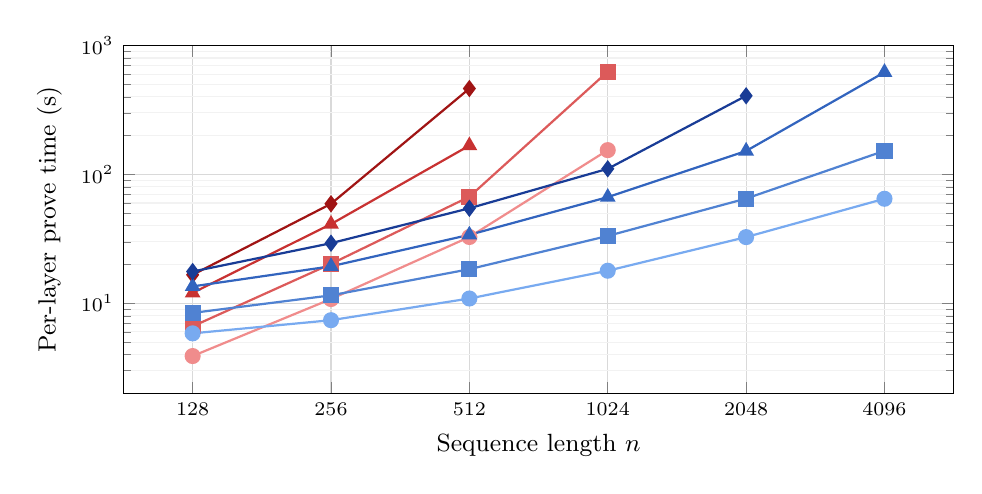
\begin{tikzpicture}
\begin{axis}[
    width=\columnwidth,
    height=6cm,
    xmode=log, ymode=log,
    log basis x=2,
    log basis y=10,
    xlabel={Sequence length $n$},
    ylabel={Per-layer prove time (s)},
    xtick={128, 256, 512, 1024, 2048, 4096},
    xticklabels={128, 256, 512, 1024, 2048, 4096},
    ymin=2, ymax=1000,
    legend to name=leg:fig6,
    legend columns=4,
    legend cell align=left,
    legend style={font=\tiny, draw=none, column sep=3pt},
    label style={font=\small},
    tick label style={font=\scriptsize},
    grid=both,
    minor grid style={gray!10},
    major grid style={gray!30},
    mark size=2.5pt,
]
% === BERT attention-only (red gradient) ===
\addplot[redspec1, mark=*, thick] coordinates {
    (128,3.90) (256,10.80) (512,32.70) (1024,154.40)
};
\addlegendentry{Tiny.Bt.}
\addplot[redspec2, mark=square*, thick] coordinates {
    (128,6.63) (256,20.23) (512,67.15) (1024,627.75)
};
\addlegendentry{Mini.Bt.}
\addplot[redspec3, mark=triangle*, thick] coordinates {
    (128,12.05) (256,41.18) (512,167.48)
};
\addlegendentry{Small.Bt.}
\addplot[redspec4, mark=diamond*, thick] coordinates {
    (128,16.65) (256,59.18) (512,463.71)
};
\addlegendentry{Base.Bt.}
% === Nystrom attention-only (blue gradient) ===
\addplot[bluespec1, mark=*, thick] coordinates {
    (128,5.85) (256,7.40) (512,10.90) (1024,17.90) (2048,32.65) (4096,64.75)
};
\addlegendentry{Tiny.Ny.}
\addplot[bluespec2, mark=square*, thick] coordinates {
    (128,8.43) (256,11.53) (512,18.40) (1024,33.33) (2048,64.98) (4096,152.43)
};
\addlegendentry{Mini.Ny.}
\addplot[bluespec3, mark=triangle*, thick] coordinates {
    (128,13.53) (256,19.38) (512,34.00) (1024,66.68) (2048,152.08) (4096,620.43)
};
\addlegendentry{Small.Ny.}
\addplot[bluespec4, mark=diamond*, thick] coordinates {
    (128,17.65) (256,29.27) (512,54.63) (1024,110.56) (2048,407.57)
};
\addlegendentry{Base.Ny.}
\end{axis}
\end{tikzpicture}\\[2pt]
\ref{leg:fig6}
\caption{Per-layer prove time for the attention equation only: BERT (red) vs.\ \nystrom (blue), log-log scale. Medium ($L{=}8$, $d{=}512$) is omitted as its per-layer cost is identical to Small ($d{=}512$).}
\label{fig:bert-vs-nystrom-freivalds}
\end{figure}

The most striking feature is the growth-rate gap: BERT's curves (red) rise steeply as $n$ increases, consistent with the $O(n^2)$ attention complexity, while \nystrom's curves (blue) grow near-linearly in the attention-only setting, reflecting $O(n)$ complexity. This translates directly into memory exhaustion: at every configuration, BERT exhausts the 128\,GB budget at a substantially shorter~$n$ than \nystrom. The feasibility gap widens as~$d$ grows: at Base ($d{=}768$, darkest shades), BERT caps at $n{=}512$ while \nystrom reaches $n{=}2048$, a $4{\times}$ extension. We omit Medium ($L{=}8$, $d{=}512$) from the figure because it yields nearly identical per-layer prove times to Small ($L{=}4$, $d{=}512$)---e.g., $167.03$\,s vs.\ $167.48$\,s for BERT at $n{=}512$---confirming the depth-invariance property: per-layer cost depends only on $d$ and $n$, not on model depth~$L$.

\sss{Quantization Fidelity}
\label{subsec:quantization-fidelity}
Table~\ref{tab:quantization} evaluates the impact of 26-bit fixed-point quantization ($k_\text{bits}{=}26$) on the pretrained uw-madison/nystromformer-512 (vocabulary size 30\,000, pretrained on BookCorpus + English Wikipedia) at sequence length $n{=}128$ over 10 batches under full cascade evaluation, where quantization errors accumulate through all 12 attention, MLP, and LayerNorm layers. The final quantized output is obtained by applying ZEN's de-quantization to the accumulated fixed-point result, and all fidelity metrics are computed on this de-quantized output. Note that the pretrained model uses $m{=}64$ landmarks (its default configuration), whereas the circuit experiments in Section~\ref{subsec:pipeline-costs} use $m{=}32$.
Top-1 agreement over all positions remains $98.8$\% and top-5 agreement is $100$\%, with cosine similarity $0.9975$. At the single \texttt{[MASK]} position the top-1 agreement drops to $90$\% but top-5 agreement stays at $100$\%, indicating that quantization primarily reshuffles near-tie predictions rather than introducing qualitatively wrong answers. These results confirm that 26-bit fixed-point arithmetic provides sufficient precision for faithful ZK-SNARK proving of transformer inference.

\begin{table}[!ht]
\centering
\caption{Quantization fidelity of 26-bit fixed-point arithmetic on a pretrained Nystr\"omformer ($d{=}768$, 12 layers, 12 heads, $m{=}64$ landmarks) at $n{=}128$.}
\label{tab:quantization}
\small
\setlength{\tabcolsep}{4pt}
\begin{tabular}{@{} ccc cc @{}}
\toprule
\multicolumn{2}{c}{Top-1 Agree.\ (\%)} & Top-5 & Cosine & RMSE \\
\cmidrule(lr){1-2}
All pos. & Mask pos. & All (\%) & Sim. & (logit) \\
\midrule
98.8 & 90.0 & 100.0 & 0.9975 & 0.378 \\
\bottomrule
\end{tabular}
\end{table}


%-------------------------------------------------------------------------------
%\subsection{Impact of Quantization on Model Predictions}
%\label{subsec:quantization-impact}
%-------------------------------------------------------------------------------
%
%\name applies 8-bit per-tensor affine quantization during ZK witness generation to enable efficient circuit representation of model weights and activations. A key question is whether this quantization meaningfully degrades model utility. To answer this, we measured the predictive behavior of the pretrained \texttt{uw-madison/nystromformer-512} model under our quantization scheme on the WikiText-103 validation set using the masked language modeling task (1{,}000 randomly sampled passages, 15\% masking rate, 15{,}122 total masked tokens, seed=42). We applied our quantization (per-tensor scale $s = (r_{\max}{-}r_{\min})/255$, zero-point $z = \mathrm{round}(-r_{\min}/s)$) to all model weights statically and to Linear and LayerNorm activations dynamically via forward hooks. Table~\ref{tab:quant-impact} summarizes the results.
%
%\begin{table}[!ht]
%\centering
%\caption{Impact of 8-bit per-tensor affine quantization on \nystromformer masked language modeling on the WikiText-103 validation set. The quantized model preserves the predictive behavior of the floating-point baseline on the vast majority of inputs.}
%\label{tab:quant-impact}
%\small
%\begin{tabular}{@{}lr@{}}
%\toprule
%\textbf{Metric} & \textbf{Value} \\
%\midrule
%Top-5 accuracy (baseline, fp32)            & 73.20\% \\
%Top-5 accuracy (quantized, 8-bit)          & 68.54\% \\
%\midrule
%Prediction agreement (top-1)               & 74.69\% \\
%Both models correct                        & 46.83\% \\
%Baseline-correct preservation rate         & 86.88\% \\
%\bottomrule
%\end{tabular}
%\end{table}
%
%Three observations support our claim that quantization preserves model utility. First, the quantized model agrees with the floating-point baseline on the top-1 prediction in 74.69\% of all masked positions, indicating that the model's predictive behavior is largely preserved at the individual prediction level. Second, among the 8{,}150 predictions where the floating-point baseline produced the correct answer, the quantized model preserved this correctness in 86.88\% of cases (7{,}081 predictions), demonstrating that quantization does not systematically degrade the model's ability to identify correct tokens. Third, the Top-5 accuracy of the quantized model (68.54\%) remains close to the floating-point baseline (73.20\%), confirming that even when the top-1 prediction shifts under quantization, the correct token typically remains within the model's high-confidence candidates. Taken together, these results indicate that the accuracy cost of our quantization scheme is bounded and does not fundamentally alter the model's predictive capability, justifying the use of 8-bit quantization for ZK circuit compatibility.

%-------------------------------------------------------------------------------
\subsection{CONCLUSION AND FUTURE WORK}
\label{subsec:discussion}
%-------------------------------------------------------------------------------
\sss{Practical impact} Our measurements across all five configurations (Figure~\ref{fig:bert-vs-nystrom-freivalds}) demonstrate that the combination of \nystrom low-rank attention and Freivalds randomized matrix-multiplication verification yields multiplicative constraint savings that translate directly into longer provable sequences. % At Base scale ($L{=}12$, $d{=}768$), \nystrom + Freivalds successfully proves all 12 attention layers up to $n{=}2048$, while BERT + Naive is limited to $n{=}128$ within the same memory budget---a $16{\times}$ gap in the maximum feasible sequence length. Note that the setup phase is a one-time circuit preparation cost amortized across all proofs of the same circuit; the per-inference proving cost is substantially smaller (e.g., $5{,}780.4$\,s for $n{=}2048$ at Base scale).

\sss{Memory as the practical bottleneck} Failed runs terminate during the Groth16 trusted setup phase, which materializes the full constraint system in RAM. Peak RSS for failed runs reaches ${\sim}118$--$122$\,GB (the effective usable limit on our 128\,GB machine), confirming that setup memory---not prover computation time---is the dominant scaling bottleneck.

\sss{The MLP frontier.} While our work removes attention as the scaling bottleneck, the feed-forward MLP block emerges as the next memory frontier. We measured the cost of proving the MLP sub-circuit---identical between BERT and \nystromformer and shared by both pipelines---and report the detailed results in Appendix~\ref{appx:mlp-costs}. The measurements confirm that, once attention is optimized, the MLP becomes the dominant constraint on the maximum provable sequence length: at $d{=}512$ and above, MLP exceeds 128\,GB at all sequence lengths including $n{=}128$. Proving full-model transformer inference at sequence lengths beyond what this work demonstrates therefore requires either reducing the MLP's per-layer constraint footprint or infrastructure-level solutions such as streaming setup, distributed proving, or GPU-accelerated SNARK libraries. We view efficient ZK proving of the MLP block as a natural follow-up direction.

\sss{Per-layer cost is depth-invariant} A consistent finding across our measurements is that per-layer attention circuit cost depends only on hidden dimension~$d$ and sequence length~$n$, not on model depth~$L$. Small ($L{=}4$, $d{=}512$) and Medium ($L{=}8$, $d{=}512$) yield identical per-layer constraints, setup, and prove time; Medium's full-model costs are exactly $2{\times}$ Small's. This depth-invariance implies that our results extrapolate to deeper architectures through simple multiplication by $L$: a 24-layer model with Base-scale dimensions would require ${\sim}2{\times}$ the prove time and setup we report for $L{=}12$. The fundamental constraint is per-layer memory, not depth.

\sss{Limitations}
Our work has several limitations. \emph{(i) Single-machine CPU-only environment.} All measurements use an Apple M1 Ultra without GPU acceleration. GPU-accelerated proving or distributed proving across multiple machines would shift relative costs, particularly for larger circuits. \emph{(ii) Trusted setup.} Our Groth16-based system requires a circuit-specific trusted setup whose memory cost is our primary scaling bottleneck. Transparent SNARKs (e.g., FRI-based or IPA-based) would eliminate this at the cost of larger proof sizes and slower verification.\emph{(iii) MLP sub-circuit.} The attention sub-circuit is made tractable by our techniques, but the MLP sub-circuit remains memory-bound at $d{\geq}256$. Proving the full transformer (attention + MLP + LayerNorm) at the scales attempted here requires further techniques for the MLP block.
%%
%% The acknowledgments section is defined using the "acks" environment
%% (and NOT an unnumbered section). This ensures the proper
%% identification of the section in the article metadata, and the
%% consistent spelling of the heading.
\begin{acks}
To Robert, for the bagels and explaining CMYK and color spaces.
\end{acks}

%%
%% The next two lines define the bibliography style to be used, and
%% the bibliography file.
\bibliographystyle{ACM-Reference-Format}
\bibliography{references}


%%
%% If your work has an appendix, this is the place to put it.
\appendix

% \section{Research Methods}

% \subsection{Part One}

% Lorem ipsum dolor sit amet, consectetur adipiscing elit. Morbi
% malesuada, quam in pulvinar varius, metus nunc fermentum urna, id
% sollicitudin purus odio sit amet enim. Aliquam ullamcorper eu ipsum
% vel mollis. Curabitur quis dictum nisl. Phasellus vel semper risus, et
% lacinia dolor. Integer ultricies commodo sem nec semper.

% \subsection{Part Two}

% Etiam commodo feugiat nisl pulvinar pellentesque. Etiam auctor sodales
% ligula, non varius nibh pulvinar semper. Suspendisse nec lectus non
% ipsum convallis congue hendrerit vitae sapien. Donec at laoreet
% eros. Vivamus non purus placerat, scelerisque diam eu, cursus
% ante. Etiam aliquam tortor auctor efficitur mattis.

% \section{Online Resources}

% Nam id fermentum dui. Suspendisse sagittis tortor a nulla mollis, in
% pulvinar ex pretium. Sed interdum orci quis metus euismod, et sagittis
% enim maximus. Vestibulum gravida massa ut felis suscipit
% congue. Quisque mattis elit a risus ultrices commodo venenatis eget
% dui. Etiam sagittis eleifend elementum.

% Nam interdum magna at lectus dignissim, ac dignissim lorem
% rhoncus. Maecenas eu arcu ac neque placerat aliquam. Nunc pulvinar
% massa et mattis lacinia.

\section{MLP + LayerNorm Circuit Costs}
\label{appx:mlp-costs}

A complete transformer layer consists of two sub-circuits: attention and the MLP\,+\,LayerNorm block. While the main text focuses on the attention sub-circuit---the target of our zkDietFormer optimizations---we additionally measured the cost of proving the MLP\,+\,LayerNorm sub-circuit, whose constraint count is the same for BERT and \nystromformer because the MLP and LayerNorm dimensions depend only on $n$ and $d$, not on the attention mechanism.
Table~\ref{tab:mlp-costs} reports per-layer average MLP\,+\,LayerNorm costs for the Tiny configuration ($L{=}2$); all timing and memory figures are the mean of the BERT and \nystrom runs.
These measurements show that the MLP\,+\,LayerNorm sub-circuit and the attention sub-circuit contribute comparable costs at $n{=}1024$: per-layer MLP\,+\,LayerNorm proving takes $516.62$\,s versus $629.29$\,s for \nystrom-Freivalds attention. The MLP\,+\,LayerNorm block consumes $112.48$\,GB peak RAM at $n{=}1024$, making it a co-bottleneck alongside attention for memory-constrained environments.

For reference, proving a complete Tiny transformer layer (attention + MLP + LayerNorm) at $n{=}1024$ requires approximately $2{,}289.03$\,s of per-layer setup and $1{,}145.91$\,s of per-layer proving (${\sim}57$\,min total per layer). We report these measurements primarily as a baseline for future work on scalable ZK proving of the full transformer layer.

\begin{table*}[!ht]
\centering
\caption{\textbf{MLP\,+\,LayerNorm} costs for the Tiny configuration ($L{=}2$, $d{=}128$).}
\label{tab:mlp-costs}
\small
\setlength{\tabcolsep}{4pt}
\begin{tabular}{@{} l rrrrrrrr @{}}
\toprule
& & & \multicolumn{2}{c}{Commit (ms)} & & & & \\
\cmidrule(lr){4-5}
$n$ & Constr.\ (M) & Setup (s) & G16 & Lasso & Prove (s) & Verify (ms) & Proof Size (KB) & Peak RAM (GB) \\
\midrule
128  & 0.98  & 94.23  & 119.3 & 147.8 & 28.38  & 285.0 & 755.8      & 26.66 \\
256  & 1.96  & 189.21 & 217.8 & 170.3 & 58.79  & 311.3 & 849.9      & 52.30 \\
512  & 3.92  & 385.63 & 441.3 & 306.0 & 137.28 & 405.5 & 1{,}026.2  & 101.93 \\
1024 & 7.84  & 883.05 & 1{,}210.3 & 433.8 & 516.62 & 482.5 & 1{,}201.7 & 112.48 \\
\bottomrule
\end{tabular}
\end{table*}

\end{document}
\endinput
%%
%% End of file `sample-sigconf.tex'.
